\newpage
\subsection{UC1: Autenticazione}
\label{UC1}
\begin{longtable}{l|p{10cm}}
\rowcolor[gray]{0.8} \multicolumn{2}{c}{} \\
\rowcolor[gray]{0.8} \multicolumn{2}{c}{\textbf{UC1 - Autenticazione}} \\
\rowcolor[gray]{0.8} \multicolumn{2}{c}{} \\
\hline
&\\
\textbf{Attori} & Utente.\\[7pt]
\textbf{Descrizione} & Il \gl{sistema} deve autenticare l'utente come ospite o come amministratore.\\[7pt]
\textbf{Precondizione} & Il sistema è stato avviato.\\[7pt]
\textbf{Postcondizione} & Il sistema ha riconosciuto l'utente come ospite o amministratore.\\[7pt]
\textbf{Scenario principale} &L'utente ha avviato il sistema per poter accedere alle funzionalità a lui dedicate.\\[7pt]
\textbf{Generalizzazioni} &UC7, UC8.\\[7pt]\hline
\end{longtable}

\subsection{UC7: Autenticazione tramite assistente virtuale}
\label{UC7}
\begin{figure}[h]
\centering
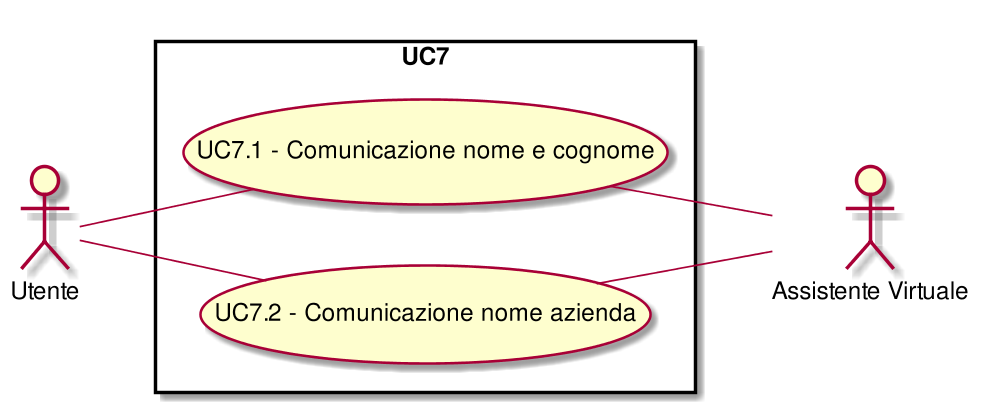
\includegraphics[width=\textwidth,height=\textheight,keepaspectratio]{images/UseCaseUC7.png}
\caption{UC7: Autenticazione tramite assistente virtuale}
\end{figure}
\begin{longtable}{l|p{10cm}}
\rowcolor[gray]{0.8} \multicolumn{2}{c}{} \\
\rowcolor[gray]{0.8} \multicolumn{2}{c}{\textbf{UC7 - Autenticazione tramite assistente virtuale}} \\
\rowcolor[gray]{0.8} \multicolumn{2}{c}{} \\
\hline
&\\
\textbf{Attori} & Assistente Virtuale, Utente.\\[7pt]
\textbf{Descrizione} & Il sistema può autenticare l'utente tramite l'assistente virtuale.\\[7pt]
\textbf{Precondizione} & L'utente utilizza direttamente l'assistente virtuale per la sua autenticazione.\\[7pt]
\textbf{Postcondizione} & Il sistema ha riconosciuto l'utente come ospite o amministratore.\\[7pt]
\textbf{Scenario principale} &L'utente viene autenticato tramite l'interazione con l'assistente virtuale.\\[7pt]
\textbf{Scenari alternativi} & Nel caso in cui nome e cognome dell'utente coincidano con quelli di un amministratore di sistema, l'assistente virtuale
richiederà all'utente l'accesso all'area di amministrazione tramite riconoscimento vocale.\\[7pt]\hline
\end{longtable}

\subsubsection{UC7.1: Comunicazione nome e cognome}
\label{UC7.1}
\begin{longtable}{l|p{10cm}}
\rowcolor[gray]{0.8} \multicolumn{2}{c}{} \\
\rowcolor[gray]{0.8} \multicolumn{2}{c}{\textbf{UC7.1 - Comunicazione nome e cognome}} \\
\rowcolor[gray]{0.8} \multicolumn{2}{c}{} \\
\hline
&\\
\textbf{Attori} & Assistente Virtuale, Utente.\\[7pt]
\textbf{Descrizione} & Il sistema può richiedere all'ospite il proprio nome e cognome per poterlo autenticare.\\[7pt]
\textbf{Precondizione} & Il sistema ha chiesto all'ospite di comunicare il proprio nome e cognome.\\[7pt]
\textbf{Postcondizione} & Il sistema ha ricevuto il nome e cognome dell'ospite.\\[7pt]
\textbf{Scenario principale} &L'utente comunica al sistema il proprio nome e cognome. \\[7pt]\hline
\end{longtable}

\subsubsection{UC7.2: Comunicazione nome azienda}
\label{UC7.2}
\begin{longtable}{l|p{10cm}}
\rowcolor[gray]{0.8} \multicolumn{2}{c}{} \\
\rowcolor[gray]{0.8} \multicolumn{2}{c}{\textbf{UC7.2 - Comunicazione nome azienda}} \\
\rowcolor[gray]{0.8} \multicolumn{2}{c}{} \\
\hline
&\\
\textbf{Attori} & Assistente Virtuale, Utente.\\[7pt]
\textbf{Descrizione} & Il sistema può richiedere all'utente il nome dell'azienda da cui proviene.\\[7pt]
\textbf{Precondizione} & Il sistema ha richiesto all'utente l'azienda da cui proviene.\\[7pt]
\textbf{Postcondizione} & Il sistema ha ricevuto dall'utente il nome dell'azienda da cui proviene.\\[7pt]
\textbf{Scenario principale} &L'utente comunica il nome dell'azienda da cui proviene.\\[7pt]\hline
\end{longtable}

\newpage
\subsection{UC8: Autenticazione tramite Slack}
\label{UC8}
\begin{longtable}{l|p{10cm}}
\rowcolor[gray]{0.8} \multicolumn{2}{c}{} \\
\rowcolor[gray]{0.8} \multicolumn{2}{c}{\textbf{UC8 - Autenticazione tramite \gl{Slack}}} \\
\rowcolor[gray]{0.8} \multicolumn{2}{c}{} \\
\hline
&\\
\textbf{Attori} & Slack, Utente.\\[7pt]
\textbf{Descrizione} & Il sistema può permettere all'utente di identificarsi come amministratore tramite Slack.\\[7pt]
\textbf{Precondizione} & L'utente vuole autenticarsi come amministratore attraverso Slack.\\[7pt]
\textbf{Postcondizione} & Il sistema identifica l'utente come amministratore del sistema.\\[7pt]
\textbf{Scenario principale} &L'utente si identifica come amministratore tramite Slack.\\[7pt]\hline
\end{longtable}

\subsection{UC9: Riconoscimento amministratore tramite assistente}
\label{UC9}
\begin{figure}[h]
\centering
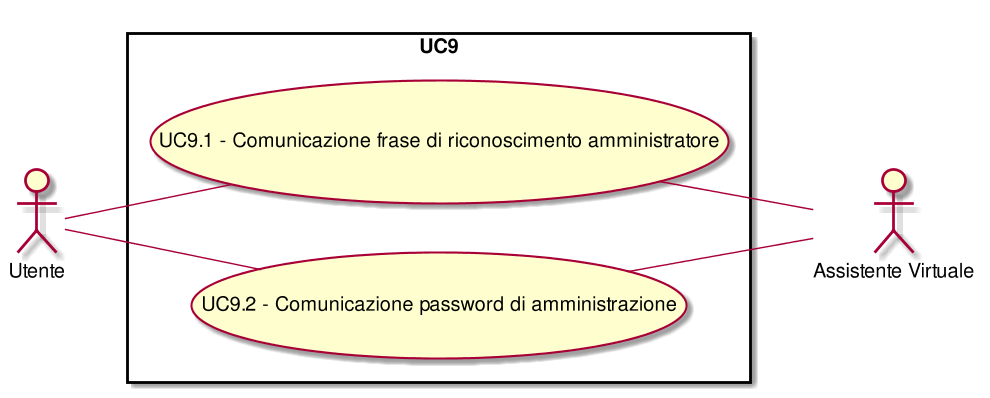
\includegraphics[width=\textwidth,height=\textheight,keepaspectratio]{images/UseCaseUC9.png}
\caption{UC9: Riconoscimento amministratore tramite assistente}
\end{figure}
\begin{longtable}{l|p{10cm}}
\rowcolor[gray]{0.8} \multicolumn{2}{c}{} \\
\rowcolor[gray]{0.8} \multicolumn{2}{c}{\textbf{UC9 - Riconoscimento amministratore tramite assistente}} \\
\rowcolor[gray]{0.8} \multicolumn{2}{c}{} \\
\hline
&\\
\textbf{Attori} & Assistente Virtuale, Utente.\\[7pt]
\textbf{Descrizione} & Il sistema offre all'utente la possibilità di autenticarsi come amministratore del sistema.\\[7pt]
\textbf{Precondizione} & Il sistema ha riconosciuto l'utente come possibile amministratore del sistema.\\[7pt]
\textbf{Postcondizione} & Il sistema ha autenticato l'utente come amministratore. \\[7pt]
\textbf{Scenario principale} &\begin{enumerate}
\item  L'utente può autenticarsi come amministratore attraverso la sua password;
\item  L'utente può autenticarsi come amministratore attraverso riconoscimento vocale.
\end{enumerate}
\\[7pt]\hline
\end{longtable}

\subsubsection{UC9.1: Comunicazione frase di riconoscimento amministratore}
\label{UC9.1}
\begin{longtable}{l|p{10cm}}
\rowcolor[gray]{0.8} \multicolumn{2}{c}{} \\
\rowcolor[gray]{0.8} \multicolumn{2}{c}{\textbf{UC9.1 - Comunicazione frase di riconoscimento amministratore}} \\
\rowcolor[gray]{0.8} \multicolumn{2}{c}{} \\
\hline
&\\
\textbf{Attori} & Assistente Virtuale, Utente.\\[7pt]
\textbf{Descrizione} & Il sistema può richiedere all'utente la frase necessaria per l'autenticazione come amministratore del sistema. \\[7pt]
\textbf{Precondizione} & Il sistema ha riconosciuto l'utente come uno dei possibili amministratori del sistema.\\[7pt]
\textbf{Postcondizione} & L'utente ha comunicato la frase necessaria per l'autenticazione come amministratore del sistema.\\[7pt]
\textbf{Scenario principale} &L'utente comunica la frase necessaria per l'autenticazione come amministratore del sistema. \\[7pt]
\textbf{Scenari alternativi} & Nel caso in cui la frase comunicata dall'utente non venga riconosciuta, il sistema richiederà nuovamente all'utente di pronunciarla.\\[7pt]\hline
\end{longtable}

\subsubsection{UC9.2: Comunicazione password di amministrazione}
\label{UC9.2}
\begin{longtable}{l|p{10cm}}
\rowcolor[gray]{0.8} \multicolumn{2}{c}{} \\
\rowcolor[gray]{0.8} \multicolumn{2}{c}{\textbf{UC9.2 - Comunicazione password di amministrazione}} \\
\rowcolor[gray]{0.8} \multicolumn{2}{c}{} \\
\hline
&\\
\textbf{Attori} & Assistente Virtuale, Utente.\\[7pt]
\textbf{Descrizione} & Il sistema offre all'utente la possibilità di autenticarsi come amministratore attraverso la sua password.\\[7pt]
\textbf{Precondizione} & Il sistema ha riconosciuto l'utente come possibile amministratore del sistema.\\[7pt]
\textbf{Postcondizione} & Il sistema ha autenticato l'utente come amministratore.\\[7pt]
\textbf{Scenario principale} &L'utente ha comunicato al sistema la sua password di amministrazione.\\[7pt]
\textbf{Scenari alternativi} & Nel caso in cui la password non sia corretta, il sistema la richiederà nuovamente.\\[7pt]\hline
\end{longtable}

\newpage\subsection{UC2: Accesso funzionalità amministratore}
\label{UC2}
\begin{figure}[h]
\centering
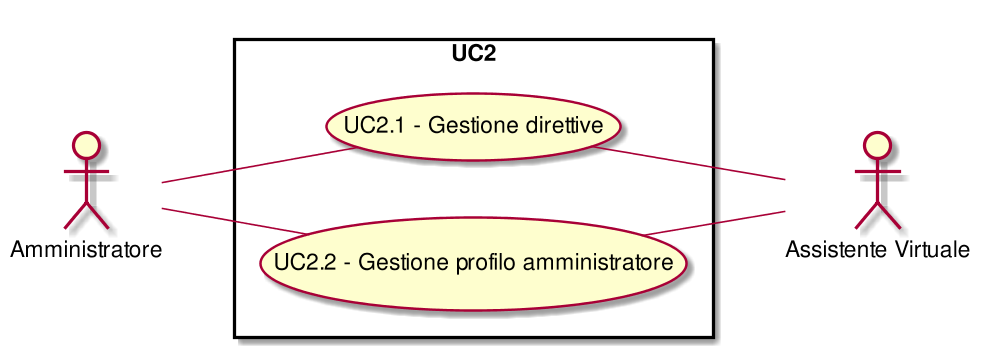
\includegraphics[width=\textwidth,height=\textheight,keepaspectratio]{images/UseCaseUC2.png}
\caption{UC2: Accesso funzionalità amministratore}
\end{figure}
\begin{longtable}{l|p{10cm}}
\rowcolor[gray]{0.8} \multicolumn{2}{c}{} \\
\rowcolor[gray]{0.8} \multicolumn{2}{c}{\textbf{UC2 - Accesso funzionalità amministratore}} \\
\rowcolor[gray]{0.8} \multicolumn{2}{c}{} \\
\hline
&\\
\textbf{Attori} & Amministratore.\\[7pt]
\textbf{Descrizione} & L'amministratore deve poter accedere alle funzionalità avanzate messe a disposizione dall'applicazione. Tali funzionalità consentono di fornire al sistema delle \gl{direttive} per modificare l'interazione con determinati ospiti, tramite un'interazione con l'assistente virtuale.\\[7pt]
\textbf{Precondizione} & L'amministratore ha effettuato l'accesso all'area di amministrazione.\\[7pt]
\textbf{Postcondizione} & L'amministratore ha usufruito delle funzionalità di amministratore fornite dal sistema.\\[7pt]
\textbf{Scenario principale} &\begin{enumerate}
\item  L'amministratore può gestire le direttive del sistema da lui accessibili;
\item  L'amministratore può gestire le informazioni del proprio profilo.
\end{enumerate}
\\[7pt]\hline
\end{longtable}

\newpage\subsubsection{UC2.1: Gestione direttive}
\label{UC2.1}
\begin{figure}[h]
\centering
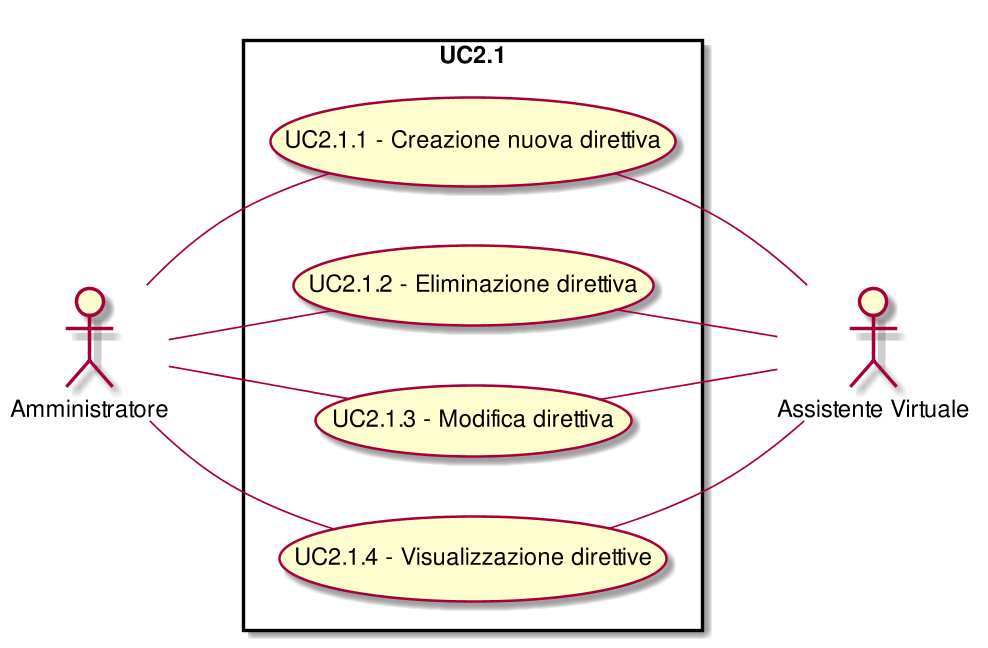
\includegraphics[width=\textwidth,height=\textheight,keepaspectratio]{images/UseCaseUC21.png}
\caption{UC2.1: Gestione direttive}
\end{figure}
\begin{longtable}{l|p{10cm}}
\rowcolor[gray]{0.8} \multicolumn{2}{c}{} \\
\rowcolor[gray]{0.8} \multicolumn{2}{c}{\textbf{UC2.1 - Gestione direttive}} \\
\rowcolor[gray]{0.8} \multicolumn{2}{c}{} \\
\hline
&\\
\textbf{Attori} & Amministratore, Assistente Virtuale.\\[7pt]
\textbf{Descrizione} & L'amministratore può creare nuove direttive o gestire quelle presenti nel sistema, tramite un'interazione con l'assistente virtuale.\\[7pt]
\textbf{Precondizione} & L'amministratore si trova nella sezione adibita alla gestione delle direttive.\\[7pt]
\textbf{Postcondizione} & L'amministratore ha usufruito delle funzionalità di gestione delle direttive.\\[7pt]
\textbf{Scenario principale} &\begin{enumerate}
\item  L'amministratore può creare una nuova \gl{direttiva};
\item  L'amministratore può eliminare una direttiva di cui ha i privilegi;
\item  L'amministratore può modificare una direttiva di cui ha i privilegi;
\item  L'amministratore può ricercare le direttive di cui ha i privilegi secondo diversi criteri (nome, funzione, target e abilitazione).
\end{enumerate}
\\[7pt]\hline
\end{longtable}

\newpage\subsubsection{UC2.1.1: Creazione nuova direttiva}
\label{UC2.1.1}
\begin{figure}[h]
\centering
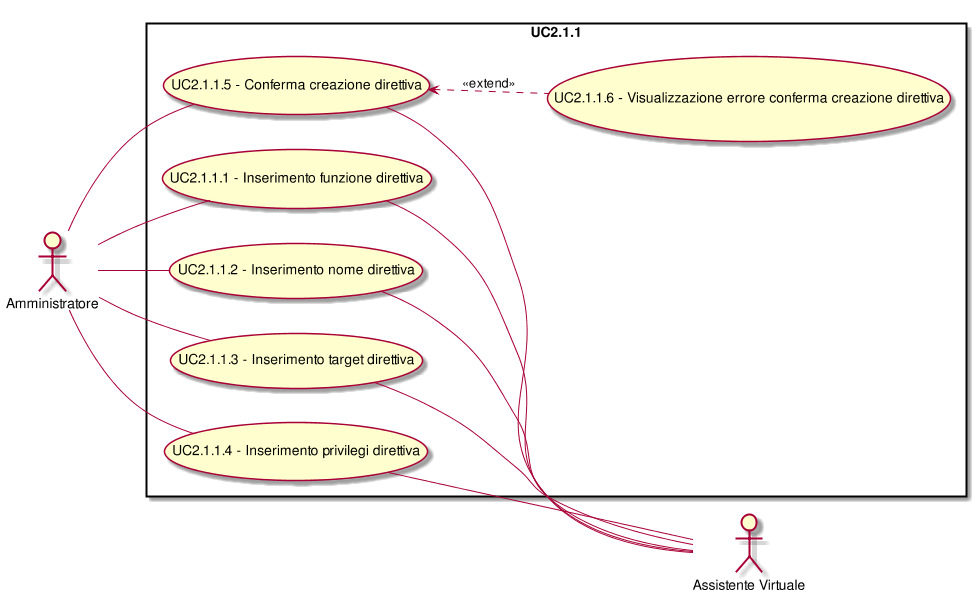
\includegraphics[width=\textwidth,height=\textheight,keepaspectratio]{images/UseCaseUC211.png}
\caption{UC2.1.1: Creazione nuova direttiva}
\end{figure}
\begin{longtable}{l|p{10cm}}
\rowcolor[gray]{0.8} \multicolumn{2}{c}{} \\
\rowcolor[gray]{0.8} \multicolumn{2}{c}{\textbf{UC2.1.1 - Creazione nuova direttiva}} \\
\rowcolor[gray]{0.8} \multicolumn{2}{c}{} \\
\hline
&\\
\textbf{Attori} & Amministratore, Assistente Virtuale.\\[7pt]
\textbf{Descrizione} & L'amministratore può creare una nuova direttiva, tramite un'interazione con l'assistente virtuale, la quale sarà salvata nel sistema.\\[7pt]
\textbf{Precondizione} & L'amministratore si trova nella sezione dedicata alla creazione di una nuova direttiva.\\[7pt]
\textbf{Postcondizione} & La direttiva è stata creata e salvata nel sistema.\\[7pt]
\textbf{Scenario principale} &\begin{enumerate}
\item  L'amministratore può inserire il nome della direttiva;
\item  L'amministratore può inserire il target della direttiva;
\item  L'amministratore può inserire la funzione della direttiva;
\item  L'amministratore può confermare la creazione della direttiva.
\end{enumerate}
\\[7pt]\hline
\end{longtable}

\newpage\subsubsection{UC2.1.1.1: Inserimento funzione direttiva}
\label{UC2.1.1.1}
\begin{longtable}{l|p{10cm}}
\rowcolor[gray]{0.8} \multicolumn{2}{c}{} \\
\rowcolor[gray]{0.8} \multicolumn{2}{c}{\textbf{UC2.1.1.1 - Inserimento funzione direttiva}} \\
\rowcolor[gray]{0.8} \multicolumn{2}{c}{} \\
\hline
&\\
\textbf{Attori} & Amministratore, Assistente Virtuale.\\[7pt]
\textbf{Descrizione} & L'amministratore può comunicare la funzione di una direttiva una volta richiesto dal sistema.\\[7pt]
\textbf{Precondizione} & Il sistema chiede all'amministratore la funzione della direttiva.\\[7pt]
\textbf{Postcondizione} & Il sistema ha ricevuto la funzione della direttiva.\\[7pt]
\textbf{Scenario principale} &L'amministratore comunica la funzione della direttiva.\\[7pt]\hline
\end{longtable}

\subsubsection{UC2.1.1.2: Inserimento nome direttiva}
\label{UC2.1.1.2}
\begin{longtable}{l|p{10cm}}
\rowcolor[gray]{0.8} \multicolumn{2}{c}{} \\
\rowcolor[gray]{0.8} \multicolumn{2}{c}{\textbf{UC2.1.1.2 - Inserimento nome direttiva}} \\
\rowcolor[gray]{0.8} \multicolumn{2}{c}{} \\
\hline
&\\
\textbf{Attori} & Amministratore, Assistente Virtuale.\\[7pt]
\textbf{Descrizione} & L'amministratore può comunicare il nome della direttiva una volta richiesto dal sistema.\\[7pt]
\textbf{Precondizione} & Il sistema ha richiesto il nome della direttiva all'amministratore.\\[7pt]
\textbf{Postcondizione} & Il sistema ha ricevuto il nome della direttiva.\\[7pt]
\textbf{Scenario principale} &L'amministratore comunica il nome della direttiva.\\[7pt]\hline
\end{longtable}

\newpage\subsubsection{UC2.1.1.3: Inserimento target direttiva}
\label{UC2.1.1.3}
\begin{figure}[h]
\centering
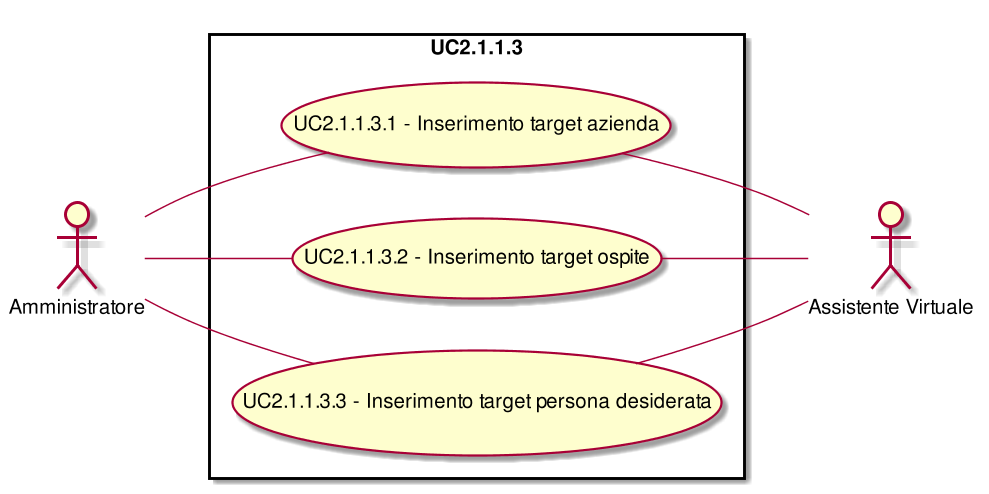
\includegraphics[width=\textwidth,height=\textheight,keepaspectratio]{images/UseCaseUC2113.png}
\caption{UC2.1.1.3: Inserimento target direttiva}
\end{figure}
\begin{longtable}{l|p{10cm}}
\rowcolor[gray]{0.8} \multicolumn{2}{c}{} \\
\rowcolor[gray]{0.8} \multicolumn{2}{c}{\textbf{UC2.1.1.3 - Inserimento target direttiva}} \\
\rowcolor[gray]{0.8} \multicolumn{2}{c}{} \\
\hline
&\\
\textbf{Attori} & Amministratore, Assistente Virtuale.\\[7pt]
\textbf{Descrizione} & L'amministratore può comunicare i target della direttiva, ovvero la categoria di persone a cui essa è rivolta, una volta richiesti dal sistema.\\[7pt]
\textbf{Precondizione} & Il sistema ha richiesto i target della direttiva all'amministratore.\\[7pt]
\textbf{Postcondizione} & Il sistema ha ricevuto i target della direttiva.\\[7pt]
\textbf{Scenario principale} &\begin{enumerate}
\item  L'amministratore può comunicare un'azienda come target;
\item  L'amministratore può comunicare il nome di un ospite come target;
\item  L'amministratore può comunicare una persona desiderata target.
\end{enumerate}
\\[7pt]\hline
\end{longtable}

\subsubsection{UC2.1.1.3.1: Inserimento target azienda}
\label{UC2.1.1.3.1}
\begin{longtable}{l|p{10cm}}
\rowcolor[gray]{0.8} \multicolumn{2}{c}{} \\
\rowcolor[gray]{0.8} \multicolumn{2}{c}{\textbf{UC2.1.1.3.1 - Inserimento target azienda}} \\
\rowcolor[gray]{0.8} \multicolumn{2}{c}{} \\
\hline
&\\
\textbf{Attori} & Amministratore, Assistente Virtuale.\\[7pt]
\textbf{Descrizione} & L'amministratore può comunicare il nome dell'azienda i cui dipendenti diventeranno i target della direttiva.\\[7pt]
\textbf{Precondizione} & Il sistema ha richiesto il nome dell'azienda target.\\[7pt]
\textbf{Postcondizione} & Il sistema ha ricevuto il nome dell'azienda target.\\[7pt]
\textbf{Scenario principale} &L'amministratore comunica il nome dell'azienda target.\\[7pt]\hline
\end{longtable}

\subsubsection{UC2.1.1.3.2: Inserimento target ospite}
\label{UC2.1.1.3.2}
\begin{longtable}{l|p{10cm}}
\rowcolor[gray]{0.8} \multicolumn{2}{c}{} \\
\rowcolor[gray]{0.8} \multicolumn{2}{c}{\textbf{UC2.1.1.3.2 - Inserimento target ospite}} \\
\rowcolor[gray]{0.8} \multicolumn{2}{c}{} \\
\hline
&\\
\textbf{Attori} & Amministratore, Assistente Virtuale.\\[7pt]
\textbf{Descrizione} & L'amministratore può comunicare il nome dell'ospite che diventerà il target della direttiva.\\[7pt]
\textbf{Precondizione} & Il sistema ha richiesto il nome dell'ospite target.\\[7pt]
\textbf{Postcondizione} & Il sistema ha ricevuto il nome dell'ospite target.\\[7pt]
\textbf{Scenario principale} &L'amministratore comunica il nome dell'ospite target.\\[7pt]\hline
\end{longtable}

\subsubsection{UC2.1.1.3.3: Inserimento target persona desiderata}
\label{UC2.1.1.3.3}
\begin{longtable}{l|p{10cm}}
\rowcolor[gray]{0.8} \multicolumn{2}{c}{} \\
\rowcolor[gray]{0.8} \multicolumn{2}{c}{\textbf{UC2.1.1.3.3 - Inserimento target persona desiderata}} \\
\rowcolor[gray]{0.8} \multicolumn{2}{c}{} \\
\hline
&\\
\textbf{Attori} & Amministratore, Assistente Virtuale.\\[7pt]
\textbf{Descrizione} & L'amministratore può comunicare il nome della persona desiderata. Tutti gli ospiti che vogliono incontrare questa persona diventeranno i target della direttiva.\\[7pt]
\textbf{Precondizione} & Il sistema ha richiesto il nome della persona desiderata.\\[7pt]
\textbf{Postcondizione} & Il sistema ha ricevuto il nome della persona desiderata.\\[7pt]
\textbf{Scenario principale} &L'amministratore comunica il nome della persona desiderata.\\[7pt]\hline
\end{longtable}

\subsubsection{UC2.1.1.4: Inserimento privilegi direttiva}
\label{UC2.1.1.4}
\begin{longtable}{l|p{10cm}}
\rowcolor[gray]{0.8} \multicolumn{2}{c}{} \\
\rowcolor[gray]{0.8} \multicolumn{2}{c}{\textbf{UC2.1.1.4 - Inserimento privilegi direttiva}} \\
\rowcolor[gray]{0.8} \multicolumn{2}{c}{} \\
\hline
&\\
\textbf{Attori} & Amministratore, Assistente Virtuale.\\[7pt]
\textbf{Descrizione} & L'amministratore può comunicare gli username degli amministratori a cui vuole concedere i privilegi di modifica ed eliminazione per la direttiva, una volta richiesti dal sistema.\\[7pt]
\textbf{Precondizione} & Il sistema ha richiesto gli username degli amministratori a cui l'amministratore vuole concedere i privilegi per la direttiva.\\[7pt]
\textbf{Postcondizione} & Il sistema ha ricevuto gli username comunicati dall'amministratore.\\[7pt]
\textbf{Scenario principale} &L'amministratore comunica gli username degli amministratori a cui vuole concedere i privilegi per la direttiva.\\[7pt]\hline
\end{longtable}

\subsubsection{UC2.1.1.5: Conferma creazione direttiva}
\label{UC2.1.1.5}
\begin{longtable}{l|p{10cm}}
\rowcolor[gray]{0.8} \multicolumn{2}{c}{} \\
\rowcolor[gray]{0.8} \multicolumn{2}{c}{\textbf{UC2.1.1.5 - Conferma creazione direttiva}} \\
\rowcolor[gray]{0.8} \multicolumn{2}{c}{} \\
\hline
&\\
\textbf{Attori} & Amministratore, Assistente Virtuale.\\[7pt]
\textbf{Descrizione} & L'amministratore può confermare i dati inseriti per creare una direttiva, una volta richiesto dal sistema.\\[7pt]
\textbf{Precondizione} & Il sistema chiede all'amministratore di confermare i dati comunicati.\\[7pt]
\textbf{Postcondizione} & Il sistema crea la direttiva con i dati comunicati dal sistema.\\[7pt]
\textbf{Scenario principale} &L'amministratore conferma di voler creare la nuova direttiva con i dati comunicati.\\[7pt]
\textbf{Scenari alternativi} & L'amministratore non conferma di voler creare la direttiva. L'amministratore viene rimandato alla pagina dedicata alla gestione delle direttive.\\[7pt]\hline
\end{longtable}

\subsubsection{UC2.1.1.6: Visualizzazione errore conferma creazione direttiva}
\label{UC2.1.1.6}
\begin{longtable}{l|p{10cm}}
\rowcolor[gray]{0.8} \multicolumn{2}{c}{} \\
\rowcolor[gray]{0.8} \multicolumn{2}{c}{\textbf{UC2.1.1.6 - Visualizzazione errore conferma creazione direttiva}} \\
\rowcolor[gray]{0.8} \multicolumn{2}{c}{} \\
\hline
&\\
\textbf{Attori} & Amministratore, Assistente Virtuale.\\[7pt]
\textbf{Descrizione} & L'amministratore può visualizzare un messaggio d'errore se ha comunicato dei dati non validi (funzione o target della direttiva inesistenti) per la creazione di una nuova direttiva.
\\[7pt]
\textbf{Precondizione} & Il sistema ha ricevuto dati non validi.\\[7pt]
\textbf{Postcondizione} & Il sistema mostra un messaggio d'errore adeguato.\\[7pt]
\textbf{Scenario principale} &L'amministratore visualizza un messaggio d'errore.\\[7pt]\hline
\end{longtable}

\newpage\subsubsection{UC2.1.2: Eliminazione direttiva }
\label{UC2.1.2}
\begin{figure}[h]
\centering

\includegraphics[width=\textwidth,height=\textheight,keepaspectratio]{images/UseCaseUC212.png}
\caption{UC2.1.2: Eliminazione direttiva }
\end{figure}
\begin{longtable}{l|p{10cm}}
\rowcolor[gray]{0.8} \multicolumn{2}{c}{} \\
\rowcolor[gray]{0.8} \multicolumn{2}{c}{\textbf{UC2.1.2 - Eliminazione direttiva }} \\
\rowcolor[gray]{0.8} \multicolumn{2}{c}{} \\
\hline
&\\
\textbf{Attori} & Amministratore, Assistente Virtuale.\\[7pt]
\textbf{Descrizione} & L'amministratore può eliminare dal sistema una direttiva di cui ha i privilegi, tramite un'interazione con l'assistente virtuale. L'eliminazione comporterà la cancellazione dei dati dal sistema.\\[7pt]
\textbf{Precondizione} & Il sistema ha richesto all'amministratore la direttiva da eliminare.\\[7pt]
\textbf{Postcondizione} & Il sistema ha ricevuto i dati della direttiva da eliminare.\\[7pt]
\textbf{Scenario principale} &L'amministratore comunica i dati della direttiva da eliminare.\\[7pt]\hline
\end{longtable}

\subsubsection{UC2.1.2.1: Conferma eliminazione direttiva}
\label{UC2.1.2.1}
\begin{longtable}{l|p{10cm}}
\rowcolor[gray]{0.8} \multicolumn{2}{c}{} \\
\rowcolor[gray]{0.8} \multicolumn{2}{c}{\textbf{UC2.1.2.1 - Conferma eliminazione direttiva}} \\
\rowcolor[gray]{0.8} \multicolumn{2}{c}{} \\
\hline
&\\
\textbf{Attori} & Amministratore, Assistente Virtuale.\\[7pt]
\textbf{Descrizione} & L'amministratore può confermare l'eliminazione di una direttiva, una volta richiesto dal sistema.\\[7pt]
\textbf{Precondizione} & Il sistema ha richiesto all'amministratore la conferma della volontà di eliminare la direttiva.\\[7pt]
\textbf{Postcondizione} & L'amministratore ha eliminato una direttiva.\\[7pt]
\textbf{Scenario principale} &L'amministratore conferma di voler eliminare la direttiva.\\[7pt]
\textbf{Scenari alternativi} & L'amministratore non conferma di voler eliminare la direttiva. L'amministratore viene rimandato alla pagina dedicata alla gestione delle direttive.\\[7pt]\hline
\end{longtable}

\newpage\subsubsection{UC2.1.3: Modifica direttiva}
\label{UC2.1.3}
\begin{figure}[h]
\centering
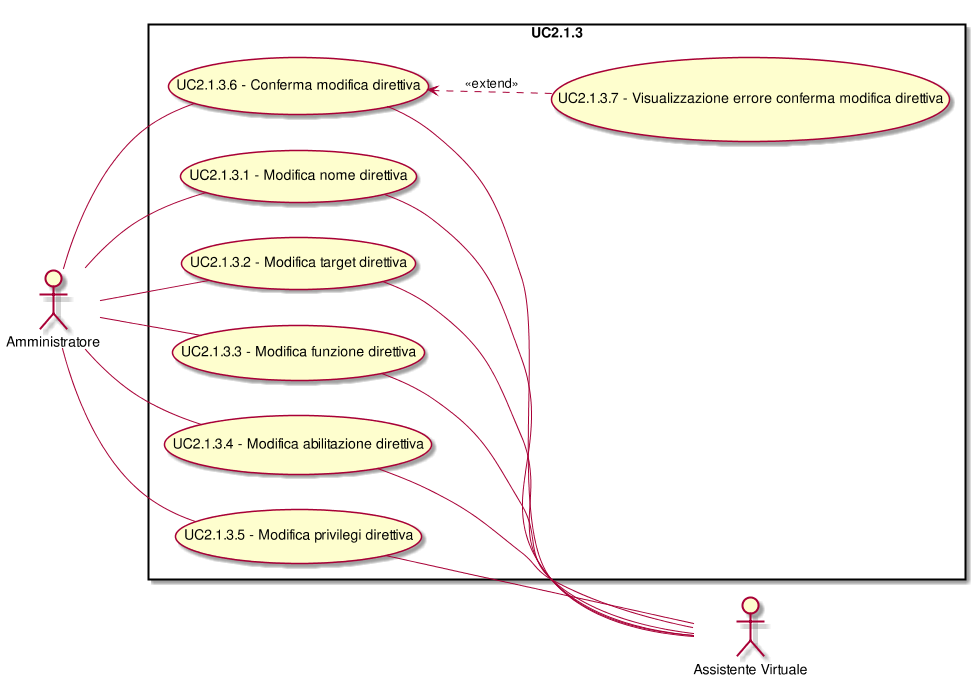
\includegraphics[width=\textwidth,height=\textheight,keepaspectratio]{images/UseCaseUC213.png}
\caption{UC2.1.3: Modifica direttiva}
\end{figure}
\begin{longtable}{l|p{10cm}}
\rowcolor[gray]{0.8} \multicolumn{2}{c}{} \\
\rowcolor[gray]{0.8} \multicolumn{2}{c}{\textbf{UC2.1.3 - Modifica direttiva}} \\
\rowcolor[gray]{0.8} \multicolumn{2}{c}{} \\
\hline
&\\
\textbf{Attori} & Amministratore, Assistente Virtuale.\\[7pt]
\textbf{Descrizione} & L'amministratore può modificare una direttiva di cui ha i privilegi, tramite un'interazione con l'assistente virtuale.\\[7pt]
\textbf{Precondizione} & Il sistema ha richiesto all'amministratore di modificare una direttiva.\\[7pt]
\textbf{Postcondizione} & Il sistema ha modificato la direttiva in base ai dati comunicati dall'amministratore.\\[7pt]
\textbf{Scenario principale} &\begin{enumerate}
\item  L'amministratore può modificare il nome della direttiva;
\item  L'amministratore può modificare il target della direttiva;
\item  L'amministratore può modificare la funzione della direttiva;
\item  L'amministratore può abilitare o disabilitare una direttiva;
\item  L'amministratore può confermare le modifiche apportate alla direttiva.
\end{enumerate}
\\[7pt]\hline
\end{longtable}

\subsubsection{UC2.1.3.1: Modifica nome direttiva}
\label{UC2.1.3.1}
\begin{longtable}{l|p{10cm}}
\rowcolor[gray]{0.8} \multicolumn{2}{c}{} \\
\rowcolor[gray]{0.8} \multicolumn{2}{c}{\textbf{UC2.1.3.1 - Modifica nome direttiva}} \\
\rowcolor[gray]{0.8} \multicolumn{2}{c}{} \\
\hline
&\\
\textbf{Attori} & Amministratore, Assistente Virtuale.\\[7pt]
\textbf{Descrizione} & L'amministratore può comunicare il nuovo nome di una direttiva.\\[7pt]
\textbf{Precondizione} & Il sistema ha chiesto all'amministratore il nuovo nome della direttiva.\\[7pt]
\textbf{Postcondizione} & Il sistema ha ricevuto i dati dall'amministratore per modificare il nome di una direttiva.\\[7pt]
\textbf{Scenario principale} &L'amministratore comunica il nuovo nome per una direttiva.\\[7pt]\hline
\end{longtable}

\newpage\subsubsection{UC2.1.3.2: Modifica target direttiva}
\label{UC2.1.3.2}
\begin{figure}[h]
\centering
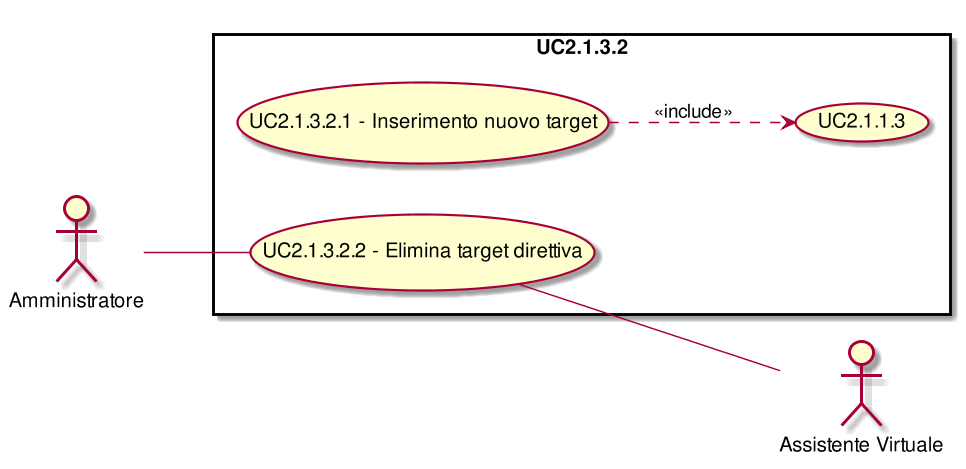
\includegraphics[width=\textwidth,height=\textheight,keepaspectratio]{images/UseCaseUC2132.png}
\caption{UC2.1.3.2: Modifica target direttiva}
\end{figure}
\begin{longtable}{l|p{10cm}}
\rowcolor[gray]{0.8} \multicolumn{2}{c}{} \\
\rowcolor[gray]{0.8} \multicolumn{2}{c}{\textbf{UC2.1.3.2 - Modifica target direttiva}} \\
\rowcolor[gray]{0.8} \multicolumn{2}{c}{} \\
\hline
&\\
\textbf{Attori} & Amministratore, Assistente Virtuale.\\[7pt]
\textbf{Descrizione} & L'amministratore può comunicare i dati per modiifcare i target di una direttiva.\\[7pt]
\textbf{Precondizione} & Il sistema ha chiesto all'amministratore il nuovo target della direttiva.\\[7pt]
\textbf{Postcondizione} & Il sistema ha ricevuto i dati dall'amministratore per modificare il target di una direttiva.\\[7pt]
\textbf{Scenario principale} &\begin{enumerate}
\item  L'amministratore può comunicare i dati per aggiungere un nuovo target alla direttiva;
\item  L'amministratore può comunicare i dati per eliminare un target dalla direttiva.
\end{enumerate}
\\[7pt]\hline
\end{longtable}

\subsubsection{UC2.1.3.2.1: Inserimento nuovo target}
\label{UC2.1.3.2.1}
\begin{longtable}{l|p{10cm}}
\rowcolor[gray]{0.8} \multicolumn{2}{c}{} \\
\rowcolor[gray]{0.8} \multicolumn{2}{c}{\textbf{UC2.1.3.2.1 - Inserimento nuovo target}} \\
\rowcolor[gray]{0.8} \multicolumn{2}{c}{} \\
\hline
&\\
\textbf{Attori} & Amministratore, Assistente Virtuale.\\[7pt]
\textbf{Descrizione} & L'amministratore può aggiungere un target alla direttiva.\\[7pt]
\textbf{Precondizione} & Il sistema ha chiesto all'amministratore il nuovo target della direttiva.\\[7pt]
\textbf{Postcondizione} & Il sistema ha ricevuto dall'amministratore il nuovo target della direttiva.\\[7pt]
\textbf{Scenario principale} &L'amministratore comunica il nuovo target della direttiva.\\[7pt]
\textbf{Inclusioni} & UC2.1.1.3\\[7pt]\hline
\end{longtable}

\subsubsection{UC2.1.3.2.2: Elimina target direttiva}
\label{UC2.1.3.2.2}
\begin{longtable}{l|p{10cm}}
\rowcolor[gray]{0.8} \multicolumn{2}{c}{} \\
\rowcolor[gray]{0.8} \multicolumn{2}{c}{\textbf{UC2.1.3.2.2 - Elimina target direttiva}} \\
\rowcolor[gray]{0.8} \multicolumn{2}{c}{} \\
\hline
&\\
\textbf{Attori} & Amministratore, Assistente Virtuale.\\[7pt]
\textbf{Descrizione} & L'amministratore può eliminare un target della direttiva.\\[7pt]
\textbf{Precondizione} & Il sistema ha chiesto all'amministratore il target da eliminare della direttiva interessata.\\[7pt]
\textbf{Postcondizione} & Il sistema ha ricevuto dall'amministratore il target da eliminare della direttiva interessata.\\[7pt]
\textbf{Scenario principale} &Il sistema riceve dall'amministratore il target da eliminare della direttiva interessata.\\[7pt]\hline
\end{longtable}

\subsubsection{UC2.1.3.3: Modifica funzione direttiva}
\label{UC2.1.3.3}
\begin{longtable}{l|p{10cm}}
\rowcolor[gray]{0.8} \multicolumn{2}{c}{} \\
\rowcolor[gray]{0.8} \multicolumn{2}{c}{\textbf{UC2.1.3.3 - Modifica funzione direttiva}} \\
\rowcolor[gray]{0.8} \multicolumn{2}{c}{} \\
\hline
&\\
\textbf{Attori} & Amministratore, Assistente Virtuale.\\[7pt]
\textbf{Descrizione} & L'amministratore può comunicare i dati per modificare la funzione di una direttiva.\\[7pt]
\textbf{Precondizione} & Il sistema ha chiesto all'amministratore la nuova funzione della direttiva.\\[7pt]
\textbf{Postcondizione} & Il sistema ha ricevuto i dati dall'amministratore per modificare la funzione di una direttiva.\\[7pt]
\textbf{Scenario principale} &L'amministratore comunica i dati per modificare la funzione di una direttiva.\\[7pt]\hline
\end{longtable}

\subsubsection{UC2.1.3.4: Modifica abilitazione direttiva}
\label{UC2.1.3.4}
\begin{longtable}{l|p{10cm}}
\rowcolor[gray]{0.8} \multicolumn{2}{c}{} \\
\rowcolor[gray]{0.8} \multicolumn{2}{c}{\textbf{UC2.1.3.4 - Modifica abilitazione direttiva}} \\
\rowcolor[gray]{0.8} \multicolumn{2}{c}{} \\
\hline
&\\
\textbf{Attori} & Amministratore, Assistente Virtuale.\\[7pt]
\textbf{Descrizione} & L'amministratore può comunicare i dati per modificare l'abilitazione di una direttiva.\\[7pt]
\textbf{Precondizione} & Il sistema ha chiesto all'amministratore come vuole modificare l'abilitazione della direttiva.\\[7pt]
\textbf{Postcondizione} & Il sistema ha ricevuto i dati dall'amministratore per modificare l'abilitazione di una direttiva.\\[7pt]
\textbf{Scenario principale} &L'amministratore comunica i dati per modificare l'abilitazione di una direttiva.\\[7pt]\hline
\end{longtable}

\subsubsection{UC2.1.3.5: Modifica privilegi direttiva}
\label{UC2.1.3.5}
\begin{figure}[h]
\centering
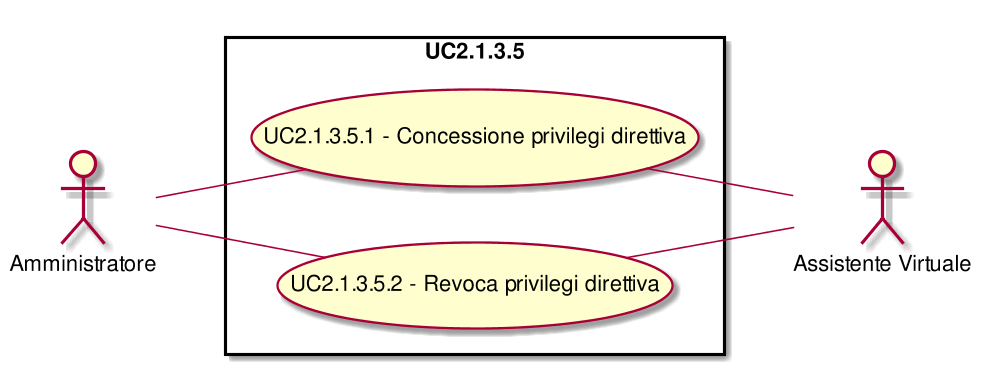
\includegraphics[width=\textwidth,height=\textheight,keepaspectratio]{images/UseCaseUC2135.png}
\caption{UC2.1.3.5: Modifica privilegi direttiva}
\end{figure}
\begin{longtable}{l|p{10cm}}
\rowcolor[gray]{0.8} \multicolumn{2}{c}{} \\
\rowcolor[gray]{0.8} \multicolumn{2}{c}{\textbf{UC2.1.3.5 - Modifica privilegi direttiva}} \\
\rowcolor[gray]{0.8} \multicolumn{2}{c}{} \\
\hline
&\\
\textbf{Attori} & Amministratore, Assistente Virtuale.\\[7pt]
\textbf{Descrizione} & L'amministratore può comunicare la volontà di modificare i privilegi per una direttiva.\\[7pt]
\textbf{Precondizione} & Il sistema ha chiesto all'amministratore se vuole modificare i privilegi di altri amministratori per la direttiva.\\[7pt]
\textbf{Postcondizione} & Il sistema ha ricevuto i dati dall'amministratore per modificare i privilegi degli altri amministratori per la direttiva.\\[7pt]
\textbf{Scenario principale} &\begin{enumerate}
\item  L'amministratore può concedere ad un altro amministratore i privilegi per una direttiva;
\item  L'amministratore può revocare i privilegi di un altro amministratore per una direttiva.
\end{enumerate}
\\[7pt]\hline
\end{longtable}

\newpage\subsubsection{UC2.1.3.5.1: Concessione privilegi direttiva}
\label{UC2.1.3.5.1}
\begin{longtable}{l|p{10cm}}
\rowcolor[gray]{0.8} \multicolumn{2}{c}{} \\
\rowcolor[gray]{0.8} \multicolumn{2}{c}{\textbf{UC2.1.3.5.1 - Concessione privilegi direttiva}} \\
\rowcolor[gray]{0.8} \multicolumn{2}{c}{} \\
\hline
&\\
\textbf{Attori} & Amministratore, Assistente Virtuale.\\[7pt]
\textbf{Descrizione} & L'amministratore può comunicare i dati per concedere ad altri amministratori i privilegi per la direttiva. L'altro amministratore in seguito potrà visualizzare, modificare ed eliminare la direttiva.\\[7pt]
\textbf{Precondizione} & Il sistema ha chiesto all'amministratore a quali altri amministratori vuole estendere i privilegi per la direttiva.\\[7pt]
\textbf{Postcondizione} & Il sistema ha ricevuto i dati dall'amministratore per concedere i privilegi di una direttiva ad ulteriori amministratori.\\[7pt]
\textbf{Scenario principale} &L'amministratore comunica i dati per concedere i privilegi per la direttiva ad altri amministratori.\\[7pt]\hline
\end{longtable}

\subsubsection{UC2.1.3.5.2: Revoca privilegi direttiva}
\label{UC2.1.3.5.2}
\begin{longtable}{l|p{10cm}}
\rowcolor[gray]{0.8} \multicolumn{2}{c}{} \\
\rowcolor[gray]{0.8} \multicolumn{2}{c}{\textbf{UC2.1.3.5.2 - Revoca privilegi direttiva}} \\
\rowcolor[gray]{0.8} \multicolumn{2}{c}{} \\
\hline
&\\
\textbf{Attori} & Amministratore, Assistente Virtuale.\\[7pt]
\textbf{Descrizione} & L'amministratore può revocare i privilegi degli altri amministratori per la direttiva.\\[7pt]
\textbf{Precondizione} & Il sistema ha chiesto all'amministratore a quali amministratori vuole revocare i privilegi per la direttiva.\\[7pt]
\textbf{Postcondizione} & Il sistema ha ricevuto gli username degli amministratori ai quali devono essere revocati i privilegi per la direttiva.\\[7pt]
\textbf{Scenario principale} &L'amministratore comunica gli username degli amministratori ai quali devono essere revocati i privilegi per la direttiva.\\[7pt]\hline
\end{longtable}

\subsubsection{UC2.1.3.6: Conferma modifica direttiva}
\label{UC2.1.3.6}
\begin{longtable}{l|p{10cm}}
\rowcolor[gray]{0.8} \multicolumn{2}{c}{} \\
\rowcolor[gray]{0.8} \multicolumn{2}{c}{\textbf{UC2.1.3.6 - Conferma modifica direttiva}} \\
\rowcolor[gray]{0.8} \multicolumn{2}{c}{} \\
\hline
&\\
\textbf{Attori} & Amministratore, Assistente Virtuale.\\[7pt]
\textbf{Descrizione} & L'amministratore può confermare la modifica di una direttiva.\\[7pt]
\textbf{Precondizione} & Il sistema ha richiesto all'amministratore la conferma delle modifiche alla direttiva.\\[7pt]
\textbf{Postcondizione} & Il sistema ha ricevuto la conferma da parte dell'amministratore.\\[7pt]
\textbf{Scenario principale} &L'amministratore conferma di voler modificare una direttiva.\\[7pt]
\textbf{Scenari alternativi} & L'amministratore non conferma di voler modificare la direttiva. L'amministratore viene rimandato alla pagina dedicata alla gestione delle direttive.\\[7pt]\hline
\end{longtable}

\subsubsection{UC2.1.3.7: Visualizzazione errore conferma modifica direttiva}
\label{UC2.1.3.7}
\begin{longtable}{l|p{10cm}}
\rowcolor[gray]{0.8} \multicolumn{2}{c}{} \\
\rowcolor[gray]{0.8} \multicolumn{2}{c}{\textbf{UC2.1.3.7 - Visualizzazione errore conferma modifica direttiva}} \\
\rowcolor[gray]{0.8} \multicolumn{2}{c}{} \\
\hline
&\\
\textbf{Attori} & Amministratore, Assistente Virtuale.\\[7pt]
\textbf{Descrizione} & L'amministratore può visualizzare un messaggio d'errore se ha comunicato dei dati non validi (target o funzione inesistenti) per la modifica di una direttiva.
\\[7pt]
\textbf{Precondizione} & Il sistema ha ricevuto dati non validi.\\[7pt]
\textbf{Postcondizione} & Il sistema mostra un messaggio d'errore.\\[7pt]
\textbf{Scenario principale} &L'amministratore visualizza un messaggio d'errore.\\[7pt]\hline
\end{longtable}

\subsubsection{UC2.1.4: Visualizzazione direttive }
\label{UC2.1.4}
\begin{longtable}{l|p{10cm}}
\rowcolor[gray]{0.8} \multicolumn{2}{c}{} \\
\rowcolor[gray]{0.8} \multicolumn{2}{c}{\textbf{UC2.1.4 - Visualizzazione direttive }} \\
\rowcolor[gray]{0.8} \multicolumn{2}{c}{} \\
\hline
&\\
\textbf{Attori} & Amministratore, Assistente Virtuale.\\[7pt]
\textbf{Descrizione} & L'amministratore può visualizzare tutte le direttive per le quali detiene i privilegi, tramite un'interazione con l'assistente virtuale.\\[7pt]
\textbf{Precondizione} & L'amministratore si trova nella sezione dedicata alla visualizzazione delle direttive.\\[7pt]
\textbf{Postcondizione} & L'amministratore ha visualizzato le direttive di cui detiene i privilegi.\\[7pt]
\textbf{Scenario principale} &L'amministratore visualizza tutte le direttive di cui detiene i privilegi.\\[7pt]\hline
\end{longtable}

\newpage\subsubsection{UC2.2: Gestione profilo amministratore}
\label{UC2.2}
\begin{figure}[h]
\centering
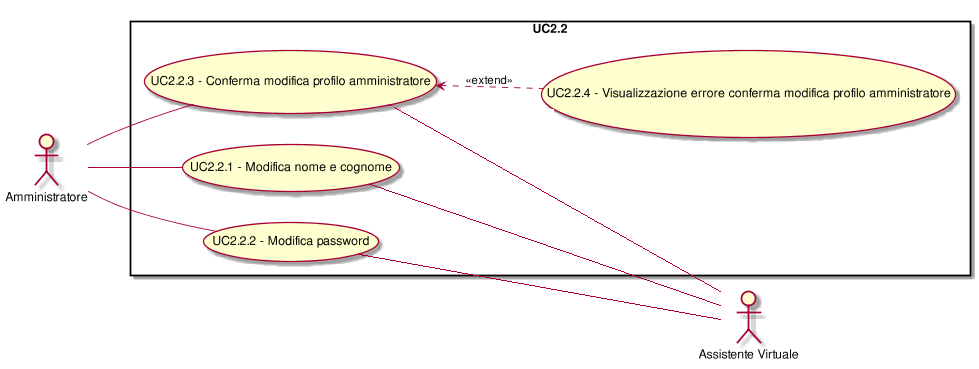
\includegraphics[width=\textwidth,height=\textheight,keepaspectratio]{images/UseCaseUC22.png}
\caption{UC2.2: Gestione profilo amministratore}
\end{figure}
\begin{longtable}{l|p{10cm}}
\rowcolor[gray]{0.8} \multicolumn{2}{c}{} \\
\rowcolor[gray]{0.8} \multicolumn{2}{c}{\textbf{UC2.2 - Gestione profilo amministratore}} \\
\rowcolor[gray]{0.8} \multicolumn{2}{c}{} \\
\hline
&\\
\textbf{Attori} & Amministratore, Assistente Virtuale.\\[7pt]
\textbf{Descrizione} & L'amministratore può gestire le impostazioni del proprio profilo, tramite un'interazione con l'assistente virtuale.\\[7pt]
\textbf{Precondizione} & L'amministratore si trova nella sezione adibita alla gestione delle impostazioni del proprio profilo.\\[7pt]
\textbf{Postcondizione} & L'amministratore ha usufruito delle funzionalità per gestire le impostazioni del proprio profilo.\\[7pt]
\textbf{Scenario principale} &\begin{enumerate}
\item  L'amministratore può modificare il proprio nome e cognome;
\item  L'amministratore può modificare la propria password;
\item  L'amministratore può confermare le modifiche effettuate.
\end{enumerate}
\\[7pt]\hline
\end{longtable}

\subsubsection{UC2.2.1: Modifica nome e cognome}
\label{UC2.2.1}
\begin{longtable}{l|p{10cm}}
\rowcolor[gray]{0.8} \multicolumn{2}{c}{} \\
\rowcolor[gray]{0.8} \multicolumn{2}{c}{\textbf{UC2.2.1 - Modifica nome e cognome}} \\
\rowcolor[gray]{0.8} \multicolumn{2}{c}{} \\
\hline
&\\
\textbf{Attori} & Amministratore, Assistente Virtuale.\\[7pt]
\textbf{Descrizione} & L'amministratore può modificare il nome e cognome del suo profilo.\\[7pt]
\textbf{Precondizione} & L'amministratore si trova nella sezione dedicata alla modifica del nome e del cognome del suo profilo.\\[7pt]
\textbf{Postcondizione} & L'amministratore ha modificato il nome e cognome del suo profilo.\\[7pt]
\textbf{Scenario principale} &L'amministratore modifica il nome e cognome del suo profilo.\\[7pt]\hline
\end{longtable}

\newpage\subsubsection{UC2.2.2: Modifica password}
\label{UC2.2.2}
\begin{figure}[h]
\centering
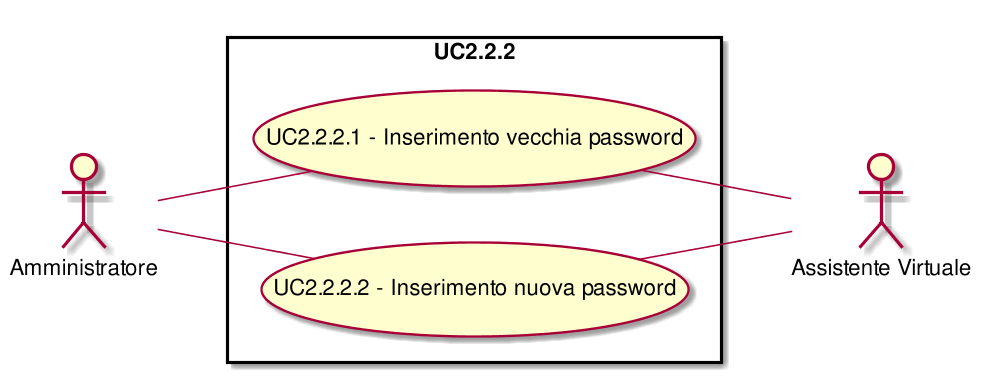
\includegraphics[width=\textwidth,height=\textheight,keepaspectratio]{images/UseCaseUC222.png}
\caption{UC2.2.2: Modifica password}
\end{figure}
\begin{longtable}{l|p{10cm}}
\rowcolor[gray]{0.8} \multicolumn{2}{c}{} \\
\rowcolor[gray]{0.8} \multicolumn{2}{c}{\textbf{UC2.2.2 - Modifica password}} \\
\rowcolor[gray]{0.8} \multicolumn{2}{c}{} \\
\hline
&\\
\textbf{Attori} & Amministratore, Assistente Virtuale.\\[7pt]
\textbf{Descrizione} & L'amministratore può modificare la password del suo profilo.\\[7pt]
\textbf{Precondizione} & L'amministratore si trova nella sezione dedicata alla modifica della password del suo profilo.\\[7pt]
\textbf{Postcondizione} & L'amministratore ha modificato la password del suo profilo.\\[7pt]
\textbf{Scenario principale} &\begin{enumerate}
\item  L'attore può inserire la propria vecchia password;
\item  L'attore può inserire una nuova password.
\end{enumerate}
\\[7pt]
\textbf{Scenari alternativi} & L'amministratore non conferma di voler modificare la propria password. L'amministratore viene rimandato alla pagina dedicata alla gestione delle direttive.\\[7pt]\hline
\end{longtable}

\subsubsection{UC2.2.2.1: Inserimento vecchia password}
\label{UC2.2.2.1}
\begin{longtable}{l|p{10cm}}
\rowcolor[gray]{0.8} \multicolumn{2}{c}{} \\
\rowcolor[gray]{0.8} \multicolumn{2}{c}{\textbf{UC2.2.2.1 - Inserimento vecchia password}} \\
\rowcolor[gray]{0.8} \multicolumn{2}{c}{} \\
\hline
&\\
\textbf{Attori} & Amministratore, Assistente Virtuale.\\[7pt]
\textbf{Descrizione} & L'amministratore può inserire la vecchia password.\\[7pt]
\textbf{Precondizione} & L'amministratore si trova nella sezione dedicata all'inserimento della vecchia password.\\[7pt]
\textbf{Postcondizione} & L'amministratore ha inserito la vecchia password.\\[7pt]
\textbf{Scenario principale} &L'amministratore inserisce la vecchia password.\\[7pt]\hline
\end{longtable}

\subsubsection{UC2.2.2.2: Inserimento nuova password}
\label{UC2.2.2.2}
\begin{longtable}{l|p{10cm}}
\rowcolor[gray]{0.8} \multicolumn{2}{c}{} \\
\rowcolor[gray]{0.8} \multicolumn{2}{c}{\textbf{UC2.2.2.2 - Inserimento nuova password}} \\
\rowcolor[gray]{0.8} \multicolumn{2}{c}{} \\
\hline
&\\
\textbf{Attori} & Amministratore, Assistente Virtuale.\\[7pt]
\textbf{Descrizione} & L'amministratore può inserire la nuova password.\\[7pt]
\textbf{Precondizione} & L'amministratore si trova nella sezione dedicata all'inserimento di una nuova password.\\[7pt]
\textbf{Postcondizione} & L'amministratore ha inserito la nuova password.\\[7pt]
\textbf{Scenario principale} &L'amministratore inserisce la nuova password.\\[7pt]\hline
\end{longtable}

\subsubsection{UC2.2.3: Conferma modifica profilo amministratore}
\label{UC2.2.3}
\begin{longtable}{l|p{10cm}}
\rowcolor[gray]{0.8} \multicolumn{2}{c}{} \\
\rowcolor[gray]{0.8} \multicolumn{2}{c}{\textbf{UC2.2.3 - Conferma modifica profilo amministratore}} \\
\rowcolor[gray]{0.8} \multicolumn{2}{c}{} \\
\hline
&\\
\textbf{Attori} & Amministratore, Assistente Virtuale.\\[7pt]
\textbf{Descrizione} & L'amministratore può confermare le modifiche al profilo.\\[7pt]
\textbf{Precondizione} & L'amministratore ha inserito i dati necessari alla modifica del profilo.\\[7pt]
\textbf{Postcondizione} & L'amministratore ha modificato il profilo.\\[7pt]
\textbf{Scenario principale} &L'amministratore modifica il profilo.\\[7pt]
\textbf{Scenari alternativi} & L'amministratore può non confermare le modifiche al profilo. Viene quindi rimandato alla pagina principale delle funzionalità di un amministratore.\\[7pt]\hline
\end{longtable}

\subsubsection{UC2.2.4: Visualizzazione errore conferma modifica profilo amministratore }
\label{UC2.2.4}
\begin{longtable}{l|p{10cm}}
\rowcolor[gray]{0.8} \multicolumn{2}{c}{} \\
\rowcolor[gray]{0.8} \multicolumn{2}{c}{\textbf{UC2.2.4 - Visualizzazione errore conferma modifica profilo amministratore }} \\
\rowcolor[gray]{0.8} \multicolumn{2}{c}{} \\
\hline
&\\
\textbf{Attori} & Amministratore, Assistente Virtuale.\\[7pt]
\textbf{Descrizione} & L'amministratore può visualizzare un messaggio d'errore se ha comunicato dei dati non validi per la modifica del profilo d'amministratore.
I dati non validi sono: username già esistente o la vecchia password non coincide con quella attuale.\\[7pt]
\textbf{Precondizione} & Il sistema ha ricevuto dati non validi.\\[7pt]
\textbf{Postcondizione} & Il sistema mostra un messaggio d'errore.\\[7pt]
\textbf{Scenario principale} &L'amministratore visualizza un messaggio d'errore.\\[7pt]\hline
\end{longtable}

\newpage\subsection{UC3: Accoglienza ospite}
\label{UC3}
\begin{figure}[h]
\centering
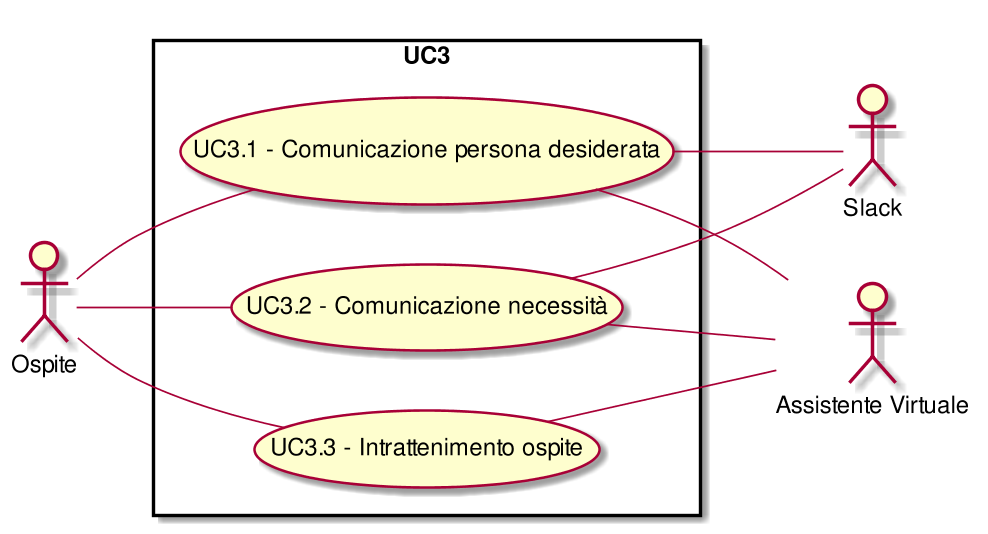
\includegraphics[width=\textwidth,height=\textheight,keepaspectratio]{images/UseCaseUC3.png}
\caption{UC3: Accoglienza ospite}
\end{figure}
\begin{longtable}{l|p{10cm}}
\rowcolor[gray]{0.8} \multicolumn{2}{c}{} \\
\rowcolor[gray]{0.8} \multicolumn{2}{c}{\textbf{UC3 - Accoglienza ospite}} \\
\rowcolor[gray]{0.8} \multicolumn{2}{c}{} \\
\hline
&\\
\textbf{Attori} & Ospite.\\[7pt]
\textbf{Descrizione} & L'ospite può essere accolto dal sistema tramite le funzionalità da esso offerte.\\[7pt]
\textbf{Precondizione} & Il sistema ha riconosciuto l'utente come ospite dell'azienda.\\[7pt]
\textbf{Postcondizione} & L'ospite è stato accolto usufruendo delle funzionalità del sistema.\\[7pt]
\textbf{Scenario principale} &\begin{enumerate}
\item  L'ospite può comunicare la persona desiderata per il suo incontro;
\item  L'ospite può esprimere alcune necessità  particolari riguardanti l'incontro;
\item  L'ospite può essere intrattenuto dal sistema durante l'attesa.
\end{enumerate}
\\[7pt]\hline
\end{longtable}

\subsubsection{UC3.1: Comunicazione persona desiderata}
\label{UC3.1}
\begin{longtable}{l|p{10cm}}
\rowcolor[gray]{0.8} \multicolumn{2}{c}{} \\
\rowcolor[gray]{0.8} \multicolumn{2}{c}{\textbf{UC3.1 - Comunicazione persona desiderata}} \\
\rowcolor[gray]{0.8} \multicolumn{2}{c}{} \\
\hline
&\\
\textbf{Attori} & Assistente Virtuale, Ospite, Slack.\\[7pt]
\textbf{Descrizione} & L'ospite può comunicare al sistema la persona che desidera incontrare.\\[7pt]
\textbf{Precondizione} & Il sistema ha richiesto all'ospite la persona desiderata per il suo incontro.\\[7pt]
\textbf{Postcondizione} & L'ospite ha comunicato al sistema la persona che vuole incontrare.\\[7pt]
\textbf{Scenario principale} &L'ospite comunica il nome della persona desiderata.\\[7pt]\hline
\end{longtable}
\newpage
\subsubsection{UC3.2: Comunicazione necessità}
\label{UC3.2}
\begin{figure}[h]
\centering
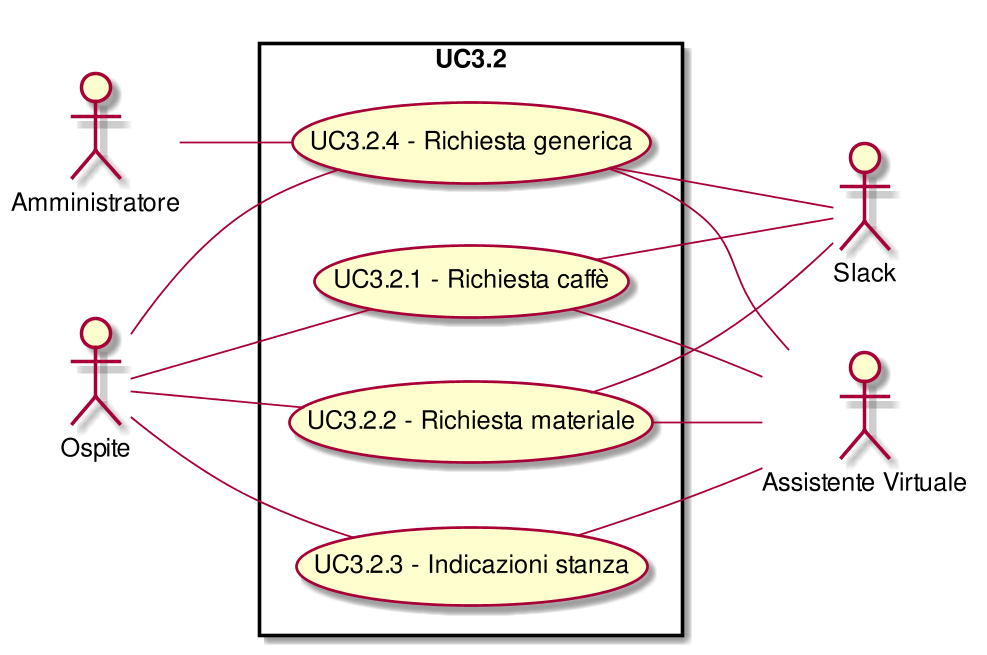
\includegraphics[width=\textwidth,height=\textheight,keepaspectratio]{images/UseCaseUC32.png}
\caption{UC3.2: Comunicazione necessità}
\end{figure}
\begin{longtable}{l|p{10cm}}
\rowcolor[gray]{0.8} \multicolumn{2}{c}{} \\
\rowcolor[gray]{0.8} \multicolumn{2}{c}{\textbf{UC3.2 - Comunicazione necessità}} \\
\rowcolor[gray]{0.8} \multicolumn{2}{c}{} \\
\hline
&\\
\textbf{Attori} & Assistente Virtuale, Ospite, Slack.\\[7pt]
\textbf{Descrizione} & Il sistema richiede all'ospite se ha particolari necessità per l'incontro.\\[7pt]
\textbf{Precondizione} & L'ospite si trova nella sezione adibita a comunicare particolari necessità riguardanti l'incontro.\\[7pt]
\textbf{Postcondizione} & Il sistema ha ricevuto le informazioni relative alle necessità dell'ospite e le ha comunicate alla persona desiderata tramite Slack.\\[7pt]
\textbf{Scenario principale} &\begin{enumerate}
\item  Il sistema può chiedere all'ospite se desidera un caffè;
\item  Il sistema può chiedere all'ospite se desidera informazioni relative alla locazione di una determinata stanza;
\item  Il sistema può chiedere all'ospite se desidera del materiale particolare per l'incontro;
\item  Il sistema può chiedere all'ospite se desidera qualche altra necessità.
\end{enumerate}
\\[7pt]\hline
\end{longtable}

\subsubsection{UC3.2.1: Richiesta caffè}
\label{UC3.2.1}
\begin{longtable}{l|p{10cm}}
\rowcolor[gray]{0.8} \multicolumn{2}{c}{} \\
\rowcolor[gray]{0.8} \multicolumn{2}{c}{\textbf{UC3.2.1 - Richiesta caffè}} \\
\rowcolor[gray]{0.8} \multicolumn{2}{c}{} \\
\hline
&\\
\textbf{Attori} & Assistente Virtuale, Ospite, Slack.\\[7pt]
\textbf{Descrizione} & Il sistema può chiedere all'ospite se desidera un caffè prima dell'incontro.\\[7pt]
\textbf{Precondizione} & Il sistema ha chiesto all'ospite se desidera un caffè.\\[7pt]
\textbf{Postcondizione} & Il sistema ha ricevuto la risposta dell'ospite, comunicandola alla persona desiderata tramite Slack.\\[7pt]
\textbf{Scenario principale} &L'ospite può comunicare di volere o meno un caffè.\\[7pt]\hline
\end{longtable}

\subsubsection{UC3.2.2: Richiesta materiale}
\label{UC3.2.2}
\begin{longtable}{l|p{10cm}}
\rowcolor[gray]{0.8} \multicolumn{2}{c}{} \\
\rowcolor[gray]{0.8} \multicolumn{2}{c}{\textbf{UC3.2.2 - Richiesta materiale}} \\
\rowcolor[gray]{0.8} \multicolumn{2}{c}{} \\
\hline
&\\
\textbf{Attori} & Assistente Virtuale, Ospite, Slack.\\[7pt]
\textbf{Descrizione} & Il sistema può chiedere all'ospite se ha bisogno di materiale particolare per l'incontro.\\[7pt]
\textbf{Precondizione} & Il sistema ha chiesto all'ospite di quale materiale ha bisogno.\\[7pt]
\textbf{Postcondizione} & Il sistema ha ricevuto i dati relativi al materiale necessario all'ospite e li ha comunicati alla persona desiderata tramite Slack.\\[7pt]
\textbf{Scenario principale} &L'ospite comunica le sue necessità riguardanti il materiale per l'incontro.\\[7pt]\hline
\end{longtable}

\newpage\subsubsection{UC3.2.3: Indicazioni stanza}
\label{UC3.2.3}
\begin{figure}[h]
\centering
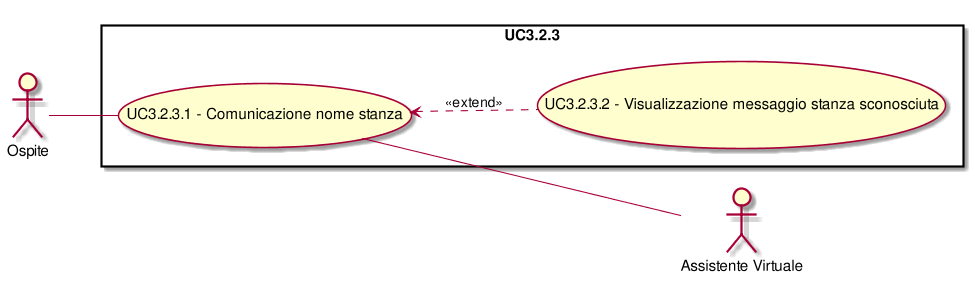
\includegraphics[width=\textwidth,height=\textheight,keepaspectratio]{images/UseCaseUC323.png}
\caption{UC3.2.3: Indicazioni stanza}
\end{figure}
\begin{longtable}{l|p{10cm}}
\rowcolor[gray]{0.8} \multicolumn{2}{c}{} \\
\rowcolor[gray]{0.8} \multicolumn{2}{c}{\textbf{UC3.2.3 - Indicazioni stanza}} \\
\rowcolor[gray]{0.8} \multicolumn{2}{c}{} \\
\hline
&\\
\textbf{Attori} & Assistente Virtuale, Ospite.\\[7pt]
\textbf{Descrizione} & Il sistema può ricevere la richiesta di informazioni relative alla locazione di una determinata stanza.\\[7pt]
\textbf{Precondizione} & L'ospite si trova nella sezione adibita a comunicare particolari necessità riguardanti l'incontro.\\[7pt]
\textbf{Postcondizione} & L'ospite ha chiesto le indicazioni.\\[7pt]
\textbf{Scenario principale} &\begin{enumerate}
\item  Il sistema chiede all'ospite il nome della stanza desiderata.
\end{enumerate}
\\[7pt]\hline
\end{longtable}

\subsubsection{UC3.2.3.1: Comunicazione nome stanza}
\label{UC3.2.3.1}
\begin{longtable}{l|p{10cm}}
\rowcolor[gray]{0.8} \multicolumn{2}{c}{} \\
\rowcolor[gray]{0.8} \multicolumn{2}{c}{\textbf{UC3.2.3.1 - Comunicazione nome stanza}} \\
\rowcolor[gray]{0.8} \multicolumn{2}{c}{} \\
\hline
&\\
\textbf{Attori} & Assistente Virtuale, Ospite.\\[7pt]
\textbf{Descrizione} & L'ospite può comunicare il nome della stanza desiderata al sistema, che mostrerà le indicazioni per raggiungerla.\\[7pt]
\textbf{Precondizione} & Il sistema ha richiesto all'ospite il nome della stanza desiderata.\\[7pt]
\textbf{Postcondizione} & Il sistema ha ricevuto il nome della stanza desiderata dall'ospite ed ha mostrato le indicazioni per raggiungerla.\\[7pt]
\textbf{Scenario principale} &Il sistema riceve il nome della stanza desiderata dall'ospite.\\[7pt]\hline
\end{longtable}

\newpage\subsubsection{UC3.2.3.2: Visualizzazione messaggio stanza sconosciuta}
\label{UC3.2.3.2}
\begin{longtable}{l|p{10cm}}
\rowcolor[gray]{0.8} \multicolumn{2}{c}{} \\
\rowcolor[gray]{0.8} \multicolumn{2}{c}{\textbf{UC3.2.3.2 - Visualizzazione messaggio stanza sconosciuta}} \\
\rowcolor[gray]{0.8} \multicolumn{2}{c}{} \\
\hline
&\\
\textbf{Attori} & Assistente Virtuale, Ospite.\\[7pt]
\textbf{Descrizione} & Il sistema può mostrare all'ospite un messaggio nel caso in cui il nome della stanza richiesta non sia riconosciuto.\\[7pt]
\textbf{Precondizione} & Il sistema ha ricevuto un nome di una stanza non presente nell'edificio.\\[7pt]
\textbf{Postcondizione} & Il sistema ha comunicato all'ospite che la stanza non è conosciuta.\\[7pt]
\textbf{Scenario principale} &Il sistema avverte l'ospite che la stanza richiesta non è conosciuta.\\[7pt]\hline
\end{longtable}

\subsubsection{UC3.2.4: Richiesta generica}
\label{UC3.2.4}
\begin{longtable}{l|p{10cm}}
\rowcolor[gray]{0.8} \multicolumn{2}{c}{} \\
\rowcolor[gray]{0.8} \multicolumn{2}{c}{\textbf{UC3.2.4 - Richiesta generica}} \\
\rowcolor[gray]{0.8} \multicolumn{2}{c}{} \\
\hline
&\\
\textbf{Attori} & Amministratore, Assistente Virtuale, Ospite, Slack.\\[7pt]
\textbf{Descrizione} & Il sistema può chiedere all'ospite altre necessità riguardanti l'incontro.\\[7pt]
\textbf{Precondizione} & Il sistema ha chiesto all'ospite se ha altre necessità per l'incontro.\\[7pt]
\textbf{Postcondizione} & Il sistema ha ricevuto i dati relativi alla necessità dell'ospite e li ha comunicati alla persona desiderata tramite Slack.\\[7pt]
\textbf{Scenario principale} &L'ospite comunica tutte le sue necessità ulteriori per l'incontro.\\[7pt]\hline
\end{longtable}

\newpage\subsubsection{UC3.3: Intrattenimento ospite}
\label{UC3.3}
\begin{figure}[h]
\centering
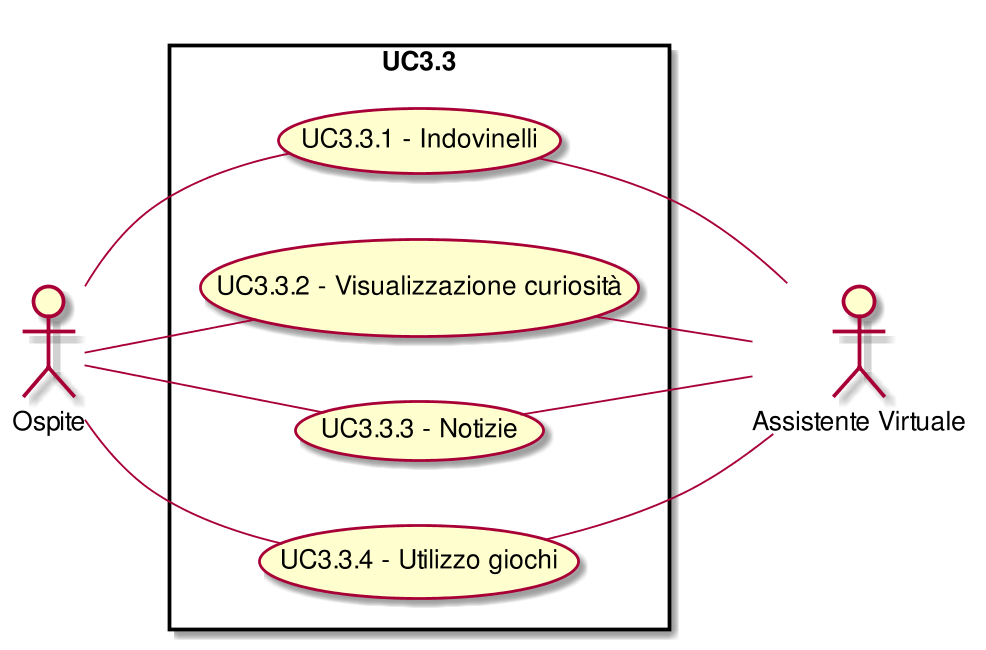
\includegraphics[width=\textwidth,height=\textheight,keepaspectratio]{images/UseCaseUC33.png}
\caption{UC3.3: Intrattenimento ospite}
\end{figure}
\begin{longtable}{l|p{10cm}}
\rowcolor[gray]{0.8} \multicolumn{2}{c}{} \\
\rowcolor[gray]{0.8} \multicolumn{2}{c}{\textbf{UC3.3 - Intrattenimento ospite}} \\
\rowcolor[gray]{0.8} \multicolumn{2}{c}{} \\
\hline
&\\
\textbf{Attori} & Assistente Virtuale, Ospite.\\[7pt]
\textbf{Descrizione} & L'ospite può scegliere tra alcuni tipi di intrattenimento forniti dal sistema, mentre attende l'arrivo della persona desiderata.\\[7pt]
\textbf{Precondizione} & L'ospite si trova nella sezione dedicata all'intrattenimento degli ospiti.\\[7pt]
\textbf{Postcondizione} & L'ospite ha usufruito degli intrattenimenti forniti dal sistema.\\[7pt]
\textbf{Scenario principale} &\begin{enumerate}
\item  L'ospite può essere intrattenuto con alcuni indovinelli ai quali deve rispondere;
\item  L'ospite può essere intrattenuto con alcune curiosità di varia natura;
\item  L'ospite può essere intrattenuto chiedendo di visualizzare alcune notizie di varia natura;
\item  L'ospite può essere intrattenuto con alcuni giochi che il sistema rende disponibili.
\end{enumerate}
\\[7pt]
\textbf{Scenari alternativi} & Dopo un certo lasso di tempo, l'ospite può sollecitare l'arrivo della persona desiderata.\\[7pt]\hline
\end{longtable}

\subsubsection{UC3.3.1: Indovinelli}
\label{UC3.3.1}
\begin{longtable}{l|p{10cm}}
\rowcolor[gray]{0.8} \multicolumn{2}{c}{} \\
\rowcolor[gray]{0.8} \multicolumn{2}{c}{\textbf{UC3.3.1 - Indovinelli}} \\
\rowcolor[gray]{0.8} \multicolumn{2}{c}{} \\
\hline
&\\
\textbf{Attori} & Assistente Virtuale, Ospite.\\[7pt]
\textbf{Descrizione} & L'ospite può rispondere ad alcuni indovinelli fatti dal sistema.\\[7pt]
\textbf{Precondizione} & L'ospite si trova nella sezione dedicata agli indovinelli.\\[7pt]
\textbf{Postcondizione} & L'ospite ha utilizzato le funzionalità degli indovinelli.\\[7pt]
\textbf{Scenario principale} &L'ospite interagisce con gli indovinelli forniti dal sistema.\\[7pt]\hline
\end{longtable}

\subsubsection{UC3.3.2: Visualizzazione curiosità}
\label{UC3.3.2}
\begin{longtable}{l|p{10cm}}
\rowcolor[gray]{0.8} \multicolumn{2}{c}{} \\
\rowcolor[gray]{0.8} \multicolumn{2}{c}{\textbf{UC3.3.2 - Visualizzazione curiosità}} \\
\rowcolor[gray]{0.8} \multicolumn{2}{c}{} \\
\hline
&\\
\textbf{Attori} & Assistente Virtuale, Ospite.\\[7pt]
\textbf{Descrizione} & L'ospite può essere intrattenuto dal sistema tramite la visualizzazione di curiosità di vario genere.\\[7pt]
\textbf{Precondizione} & L'ospite si trova nella sezione dedicata alla visualizzazione delle curiosità.\\[7pt]
\textbf{Postcondizione} & L'ospite ha visualizzato alcune curiosità.\\[7pt]
\textbf{Scenario principale} &L'ospite visualizza le curiosità fornite dal sistema.\\[7pt]\hline
\end{longtable}

\newpage\subsubsection{UC3.3.3: Notizie}
\label{UC3.3.3}
\begin{figure}[h]
\centering
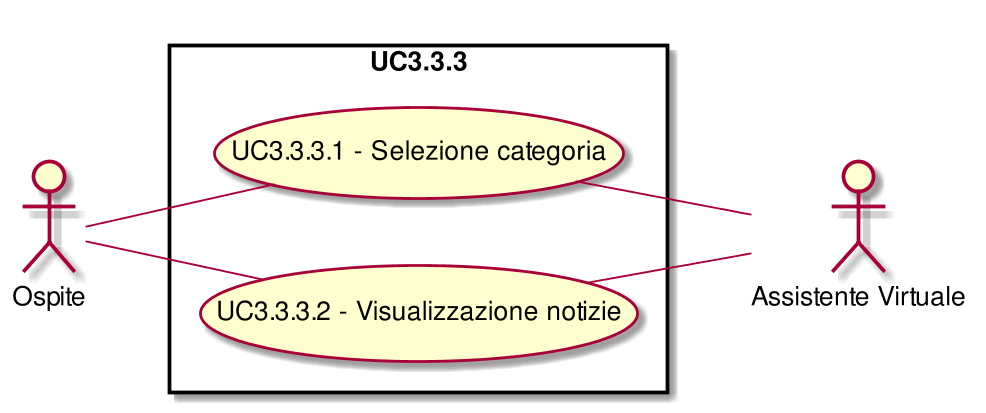
\includegraphics[width=\textwidth,height=\textheight,keepaspectratio]{images/UseCaseUC333.png}
\caption{UC3.3.3: Notizie}
\end{figure}
\begin{longtable}{l|p{10cm}}
\rowcolor[gray]{0.8} \multicolumn{2}{c}{} \\
\rowcolor[gray]{0.8} \multicolumn{2}{c}{\textbf{UC3.3.3 - Notizie}} \\
\rowcolor[gray]{0.8} \multicolumn{2}{c}{} \\
\hline
&\\
\textbf{Attori} & Assistente Virtuale, Ospite.\\[7pt]
\textbf{Descrizione} & L'ospite può essere intrattenuto chiedendo di visualizzare le ultime notizie riguardanti categorie di vario genere.\\[7pt]
\textbf{Precondizione} & L'ospite si trova nella sezione dedicata alla visualizzazione delle notizie.\\[7pt]
\textbf{Postcondizione} & L'ospite ha visualizzato le notizie da lui richieste.\\[7pt]
\textbf{Scenario principale} &L'ospite visualizza le notizie riguardanti la categoria richiesta.\\[7pt]\hline
\end{longtable}

\subsubsection{UC3.3.3.1: Selezione categoria}
\label{UC3.3.3.1}
\begin{longtable}{l|p{10cm}}
\rowcolor[gray]{0.8} \multicolumn{2}{c}{} \\
\rowcolor[gray]{0.8} \multicolumn{2}{c}{\textbf{UC3.3.3.1 - Selezione categoria}} \\
\rowcolor[gray]{0.8} \multicolumn{2}{c}{} \\
\hline
&\\
\textbf{Attori} & Assistente Virtuale, Ospite.\\[7pt]
\textbf{Descrizione} & Il sistema permette all'utente di selezionare la categoria di notizie da visualizzare.\\[7pt]
\textbf{Precondizione} & Il sistema ha richiesto all'ospite di selezionare la categoria di notizie.\\[7pt]
\textbf{Postcondizione} & L'ospite ha specificato la categoria di notizie alla quale è interessato.\\[7pt]
\textbf{Scenario principale} &L'ospite comunica al sistema la di categoria desiderata.\\[7pt]\hline
\end{longtable}

\subsubsection{UC3.3.3.2: Visualizzazione notizie}
\label{UC3.3.3.2}
\begin{longtable}{l|p{10cm}}
\rowcolor[gray]{0.8} \multicolumn{2}{c}{} \\
\rowcolor[gray]{0.8} \multicolumn{2}{c}{\textbf{UC3.3.3.2 - Visualizzazione notizie}} \\
\rowcolor[gray]{0.8} \multicolumn{2}{c}{} \\
\hline
&\\
\textbf{Attori} & Assistente Virtuale, Ospite.\\[7pt]
\textbf{Descrizione} & L'ospite può visualizzare le notizie fornite dal sistema.\\[7pt]
\textbf{Precondizione} & Il sistema ricevuto dall'ospite la categoria di notizie che desidera visualizzare.\\[7pt]
\textbf{Postcondizione} & Il sistema ha mostrato all'utente una notizia della categoria richiesta.\\[7pt]
\textbf{Scenario principale} &L'ospite visualizza la notizia fornita dal sistema.\\[7pt]\hline
\end{longtable}

\subsubsection{UC3.3.4: Utilizzo giochi}
\label{UC3.3.4}
\begin{figure}[h]
\centering
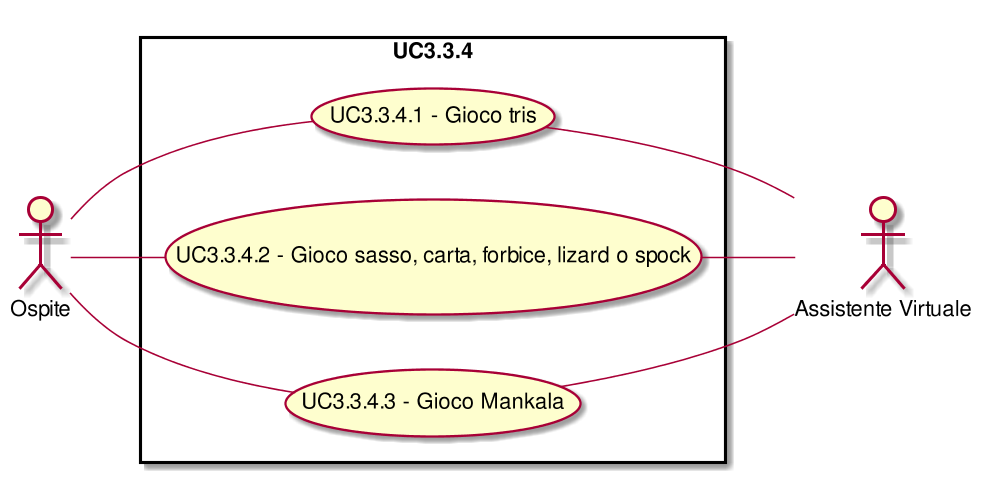
\includegraphics[width=\textwidth,height=\textheight,keepaspectratio]{images/UseCaseUC334.png}
\caption{UC3.3.4: Utilizzo giochi}
\end{figure}
\begin{longtable}{l|p{10cm}}
\rowcolor[gray]{0.8} \multicolumn{2}{c}{} \\
\rowcolor[gray]{0.8} \multicolumn{2}{c}{\textbf{UC3.3.4 - Utilizzo giochi}} \\
\rowcolor[gray]{0.8} \multicolumn{2}{c}{} \\
\hline
&\\
\textbf{Attori} & Assistente Virtuale, Ospite.\\[7pt]
\textbf{Descrizione} & L'ospite può essere intrattenuto tramite alcuni giochi forniti dal sistema.\\[7pt]
\textbf{Precondizione} & L'ospite si trova nella sezione dedicata ai giochi.\\[7pt]
\textbf{Postcondizione} & L'ospite ha interagito con i giochi forniti dal sistema.\\[7pt]
\textbf{Scenario principale} &L'ospite interagisce con i giochi forniti dal sistema.\\[7pt]\hline
\end{longtable}

\newpage\subsubsection{UC3.3.4.1: Gioco tris}
\label{UC3.3.4.1}
\begin{figure}[h]
\centering
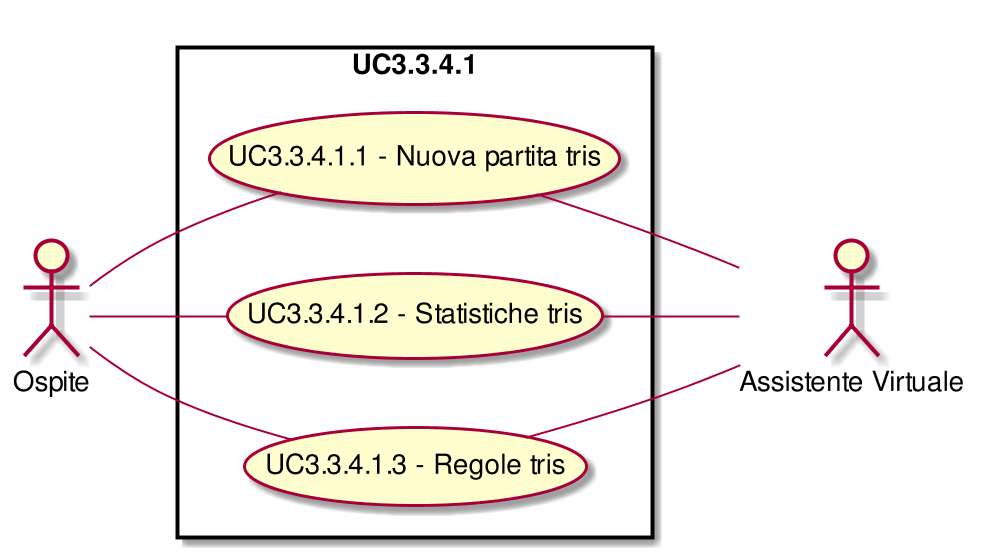
\includegraphics[width=\textwidth,height=\textheight,keepaspectratio]{images/UseCaseUC3341.png}
\caption{UC3.3.4.1: Gioco tris}
\end{figure}
\begin{longtable}{l|p{10cm}}
\rowcolor[gray]{0.8} \multicolumn{2}{c}{} \\
\rowcolor[gray]{0.8} \multicolumn{2}{c}{\textbf{UC3.3.4.1 - Gioco tris}} \\
\rowcolor[gray]{0.8} \multicolumn{2}{c}{} \\
\hline
&\\
\textbf{Attori} & Assistente Virtuale, Ospite.\\[7pt]
\textbf{Descrizione} & Il sistema può permettere all'ospite di giocare a tris.\\[7pt]
\textbf{Precondizione} & L'ospite si trova nella sezione dedicata al gioco del tris.\\[7pt]
\textbf{Postcondizione} & L'ospite ha terminato una partita a tris contro il sistema.\\[7pt]
\textbf{Scenario principale} &L'utente gioca una partita di tris contro il sistema.\\[7pt]\hline
\end{longtable}

\subsubsection{UC3.3.4.1.1: Nuova partita tris}
\label{UC3.3.4.1.1}
\begin{longtable}{l|p{10cm}}
\rowcolor[gray]{0.8} \multicolumn{2}{c}{} \\
\rowcolor[gray]{0.8} \multicolumn{2}{c}{\textbf{UC3.3.4.1.1 - Nuova partita tris}} \\
\rowcolor[gray]{0.8} \multicolumn{2}{c}{} \\
\hline
&\\
\textbf{Attori} & Assistente Virtuale, Ospite.\\[7pt]
\textbf{Descrizione} & Il sistema può permettere all'ospite di iniziare una nuova partita a tris.\\[7pt]
\textbf{Precondizione} & Il sistema ha avviato il gioco tris.
\\[7pt]
\textbf{Postcondizione} & Il sistema ha avviato una nuova partita di tris.
\\[7pt]
\textbf{Scenario principale} &L'ospite chiede al sistema di iniziare una nuova partita a tris.\\[7pt]\hline
\end{longtable}

\subsubsection{UC3.3.4.1.2: Statistiche tris}
\label{UC3.3.4.1.2}
\begin{longtable}{l|p{10cm}}
\rowcolor[gray]{0.8} \multicolumn{2}{c}{} \\
\rowcolor[gray]{0.8} \multicolumn{2}{c}{\textbf{UC3.3.4.1.2 - Statistiche tris}} \\
\rowcolor[gray]{0.8} \multicolumn{2}{c}{} \\
\hline
&\\
\textbf{Attori} & Assistente Virtuale, Ospite.\\[7pt]
\textbf{Descrizione} & Il sistema può offrire all'ospite la possibilità di visualizzare le statistiche delle partite.\\[7pt]
\textbf{Precondizione} & Il sistema ha avviato il gioco tris.\\[7pt]
\textbf{Postcondizione} & Il sistema ha mostrato le statistiche delle partite all'ospite.\\[7pt]
\textbf{Scenario principale} &L'ospite ha richiesto di visualizzare le statistiche delle partite.\\[7pt]\hline
\end{longtable}

\subsubsection{UC3.3.4.1.3: Regole tris}
\label{UC3.3.4.1.3}
\begin{longtable}{l|p{10cm}}
\rowcolor[gray]{0.8} \multicolumn{2}{c}{} \\
\rowcolor[gray]{0.8} \multicolumn{2}{c}{\textbf{UC3.3.4.1.3 - Regole tris}} \\
\rowcolor[gray]{0.8} \multicolumn{2}{c}{} \\
\hline
&\\
\textbf{Attori} & Assistente Virtuale, Ospite.\\[7pt]
\textbf{Descrizione} & Il sistema può permettere all'ospite di visualizzare le regole del gioco tris.\\[7pt]
\textbf{Precondizione} & Il sistema ha avviato il gioco tris.\\[7pt]
\textbf{Postcondizione} & Il sistema ha mostrato all'ospite le regole del gioco tris.\\[7pt]
\textbf{Scenario principale} &L'ospite chiede le regole del gioco tris.\\[7pt]\hline
\end{longtable}

\newpage\subsubsection{UC3.3.4.2: Gioco sasso, carta, forbice, lizard o spock}
\label{UC3.3.4.2}
\begin{figure}[h]
\centering
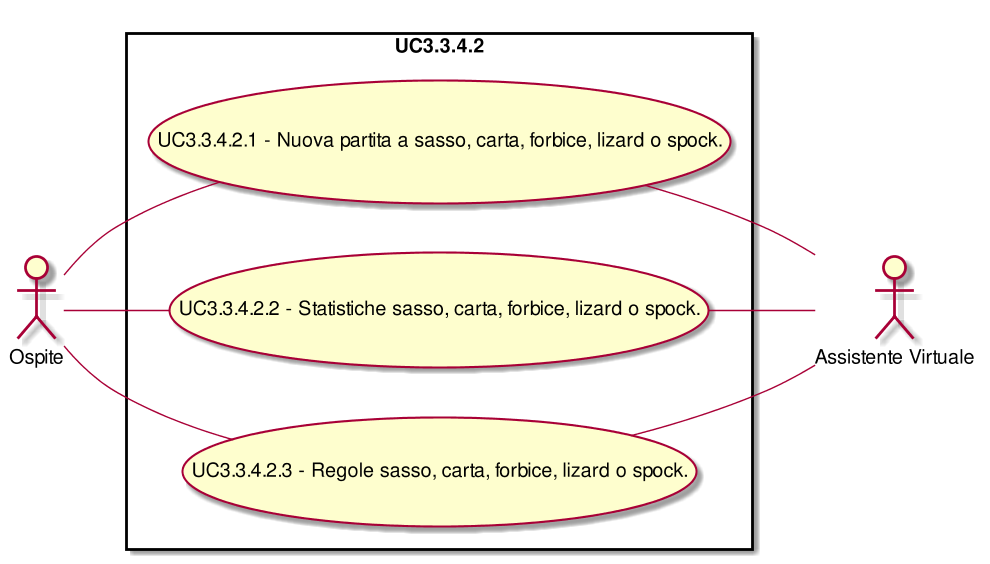
\includegraphics[width=\textwidth,height=\textheight,keepaspectratio]{images/UseCaseUC3342.png}
\caption{UC3.3.4.2: Gioco sasso, carta, forbice, lizard o spock}
\end{figure}
\begin{longtable}{l|p{10cm}}
\rowcolor[gray]{0.8} \multicolumn{2}{c}{} \\
\rowcolor[gray]{0.8} \multicolumn{2}{c}{\textbf{UC3.3.4.2 - Gioco sasso, carta, forbice, lizard o spock}} \\
\rowcolor[gray]{0.8} \multicolumn{2}{c}{} \\
\hline
&\\
\textbf{Attori} & Assistente Virtuale, Ospite.\\[7pt]
\textbf{Descrizione} & Il sistema può permettere all'ospite di giocare a  sasso, carta, forbice, lizard o spock.\\[7pt]
\textbf{Precondizione} & L'ospite si trova nella sezione dedicata al gioco sasso, carta, forbice, lizard o spock.\\[7pt]
\textbf{Postcondizione} & L'ospite ha terminato una partita a sasso, carta, forbice, lizard o spock contro il sistema.\\[7pt]
\textbf{Scenario principale} &L'utente gioca una partita a sasso, carta, forbice, lizard o spock contro il sistema.\\[7pt]\hline
\end{longtable}

\subsubsection{UC3.3.4.2.1: Nuova partita a sasso, carta, forbice, lizard o spock.}
\label{UC3.3.4.2.1}
\begin{longtable}{l|p{10cm}}
\rowcolor[gray]{0.8} \multicolumn{2}{c}{} \\
\rowcolor[gray]{0.8} \multicolumn{2}{c}{\textbf{UC3.3.4.2.1 - Nuova partita a sasso, carta, forbice, lizard o spock.}} \\
\rowcolor[gray]{0.8} \multicolumn{2}{c}{} \\
\hline
&\\
\textbf{Attori} & Assistente Virtuale, Ospite.\\[7pt]
\textbf{Descrizione} & Il sistema può permettere all'ospite di iniziare una nuova partita a sasso, carta, forbice, lizard o spock.\\[7pt]
\textbf{Precondizione} & Il sistema ha avviato il gioco sasso, carta, forbice, lizard o spock.\\[7pt]
\textbf{Postcondizione} & Il sistema ha avviato una nuova partita a sasso, carta, forbice, lizard o spock.\\[7pt]
\textbf{Scenario principale} &L'ospite chiede al sistema di iniziare una nuova partita a sasso, carta, forbice, lizard o spock.\\[7pt]\hline
\end{longtable}

\subsubsection{UC3.3.4.2.2: Statistiche sasso, carta, forbice, lizard o spock.}
\label{UC3.3.4.2.2}
\begin{longtable}{l|p{10cm}}
\rowcolor[gray]{0.8} \multicolumn{2}{c}{} \\
\rowcolor[gray]{0.8} \multicolumn{2}{c}{\textbf{UC3.3.4.2.2 - Statistiche sasso, carta, forbice, lizard o spock.}} \\
\rowcolor[gray]{0.8} \multicolumn{2}{c}{} \\
\hline
&\\
\textbf{Attori} & Assistente Virtuale, Ospite.\\[7pt]
\textbf{Descrizione} & Il sistema può offrire all'ospite la possibilità di visualizzare le statistiche delle partite.\\[7pt]
\textbf{Precondizione} & Il sistema ha avviato il gioco sasso, carta, forbice, lizard o spock.\\[7pt]
\textbf{Postcondizione} & Il sistema ha mostrato le statistiche delle partite all'ospite.\\[7pt]
\textbf{Scenario principale} &L'ospite ha richiesto di visualizzare le statistiche delle partite.\\[7pt]\hline
\end{longtable}

\subsubsection{UC3.3.4.2.3: Regole sasso, carta, forbice, lizard o spock.}
\label{UC3.3.4.2.3}
\begin{longtable}{l|p{10cm}}
\rowcolor[gray]{0.8} \multicolumn{2}{c}{} \\
\rowcolor[gray]{0.8} \multicolumn{2}{c}{\textbf{UC3.3.4.2.3 - Regole sasso, carta, forbice, lizard o spock.}} \\
\rowcolor[gray]{0.8} \multicolumn{2}{c}{} \\
\hline
&\\
\textbf{Attori} & Assistente Virtuale, Ospite.\\[7pt]
\textbf{Descrizione} & Il sistema può permettere all'ospite di visualizzare le regole del gioco sasso, carta, forbice, lizard o spock.\\[7pt]
\textbf{Precondizione} & Il sistema ha avviato il gioco sasso, carta, forbice, lizard o spock.\\[7pt]
\textbf{Postcondizione} & Il sistema ha mostrato all'ospite le regole del gioco sasso, carta, forbice, lizard o spock.\\[7pt]
\textbf{Scenario principale} &L'ospite chiede le regole del gioco sasso, carta, forbice, lizard o spock.\\[7pt]\hline
\end{longtable}

\newpage\subsubsection{UC3.3.4.3: Gioco Mankala}
\label{UC3.3.4.3}
\begin{figure}[h]
\centering
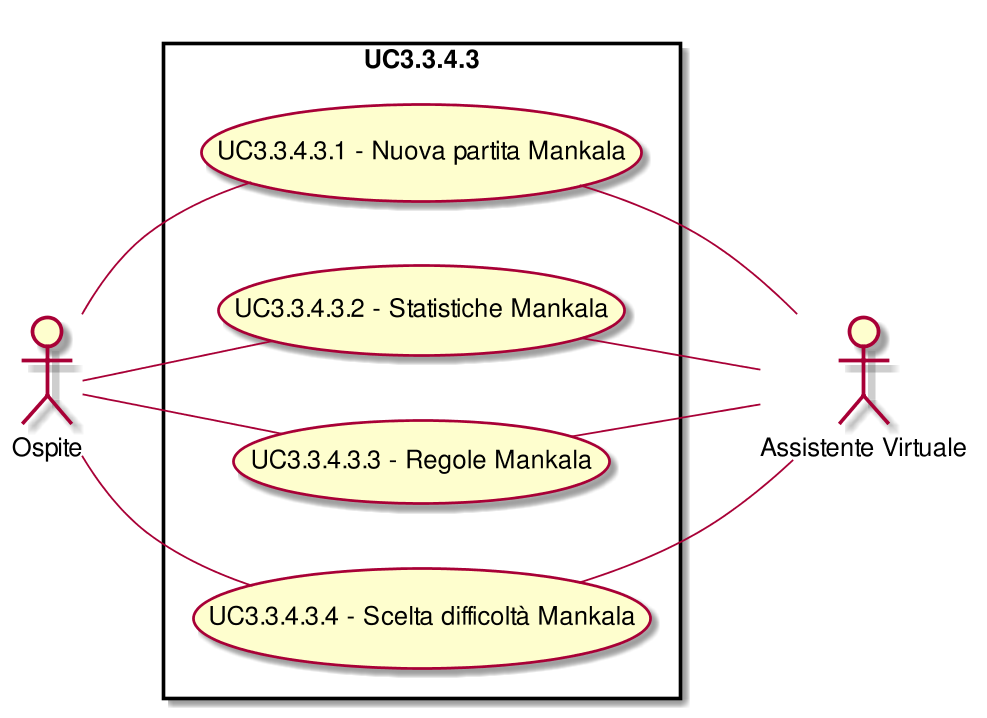
\includegraphics[width=\textwidth,height=\textheight,keepaspectratio]{images/UseCaseUC3343.png}
\caption{UC3.3.4.3: Gioco Mankala}
\end{figure}
\begin{longtable}{l|p{10cm}}
\rowcolor[gray]{0.8} \multicolumn{2}{c}{} \\
\rowcolor[gray]{0.8} \multicolumn{2}{c}{\textbf{UC3.3.4.3 - Gioco Mankala}} \\
\rowcolor[gray]{0.8} \multicolumn{2}{c}{} \\
\hline
&\\
\textbf{Attori} & Assistente Virtuale, Ospite.\\[7pt]
\textbf{Descrizione} & Il sistema può permettere all'ospite di giocare a Mankala.\\[7pt]
\textbf{Precondizione} & L'ospite si trova nella sezione dedicata al gioco Mankala.\\[7pt]
\textbf{Postcondizione} & L'ospite ha terminato una partita a Mankala contro il sistema.\\[7pt]
\textbf{Scenario principale} &L'ospite gioca una partita a Mankala contro il sistema.\\[7pt]\hline
\end{longtable}

\subsubsection{UC3.3.4.3.1: Nuova partita Mankala}
\label{UC3.3.4.3.1}
\begin{longtable}{l|p{10cm}}
\rowcolor[gray]{0.8} \multicolumn{2}{c}{} \\
\rowcolor[gray]{0.8} \multicolumn{2}{c}{\textbf{UC3.3.4.3.1 - Nuova partita Mankala}} \\
\rowcolor[gray]{0.8} \multicolumn{2}{c}{} \\
\hline
&\\
\textbf{Attori} & Assistente Virtuale, Ospite.\\[7pt]
\textbf{Descrizione} & Il sistema può permettere all'ospite di iniziare una nuova partita a Mankala.\\[7pt]
\textbf{Precondizione} & Il sistema ha avviato il gioco Mankala.\\[7pt]
\textbf{Postcondizione} & Il sistema ha avviato una nuova partita di Mankala.\\[7pt]
\textbf{Scenario principale} &L'ospite chiede al sistema di iniziare una nuova partita a Mankala.\\[7pt]\hline
\end{longtable}

\subsubsection{UC3.3.4.3.2: Statistiche Mankala}
\label{UC3.3.4.3.2}
\begin{longtable}{l|p{10cm}}
\rowcolor[gray]{0.8} \multicolumn{2}{c}{} \\
\rowcolor[gray]{0.8} \multicolumn{2}{c}{\textbf{UC3.3.4.3.2 - Statistiche Mankala}} \\
\rowcolor[gray]{0.8} \multicolumn{2}{c}{} \\
\hline
&\\
\textbf{Attori} & Assistente Virtuale, Ospite.\\[7pt]
\textbf{Descrizione} & Il sistema può offrire all'ospite la possibilità di visualizzare le statistiche delle partite.\\[7pt]
\textbf{Precondizione} & Il sistema ha avviato il gioco Mankala.\\[7pt]
\textbf{Postcondizione} & Il sistema ha mostrato le statistiche delle partite all'ospite.\\[7pt]
\textbf{Scenario principale} &L'ospite ha richiesto di visualizzare le statistiche delle partite.\\[7pt]\hline
\end{longtable}

\subsubsection{UC3.3.4.3.3: Regole Mankala}
\label{UC3.3.4.3.3}
\begin{longtable}{l|p{10cm}}
\rowcolor[gray]{0.8} \multicolumn{2}{c}{} \\
\rowcolor[gray]{0.8} \multicolumn{2}{c}{\textbf{UC3.3.4.3.3 - Regole Mankala}} \\
\rowcolor[gray]{0.8} \multicolumn{2}{c}{} \\
\hline
&\\
\textbf{Attori} & Assistente Virtuale, Ospite.\\[7pt]
\textbf{Descrizione} & Il sistema può permettere all'ospite di visualizzare le regole del gioco Mankala.\\[7pt]
\textbf{Precondizione} & Il sistema ha avviato il gioco Mankala.\\[7pt]
\textbf{Postcondizione} & Il sistema ha mostrato all'ospite le regole del gioco Mankala.\\[7pt]
\textbf{Scenario principale} &L'ospite chiede le regole del gioco Mankala.\\[7pt]\hline
\end{longtable}

\subsubsection{UC3.3.4.3.4: Scelta difficoltà Mankala}
\label{UC3.3.4.3.4}
\begin{longtable}{l|p{10cm}}
\rowcolor[gray]{0.8} \multicolumn{2}{c}{} \\
\rowcolor[gray]{0.8} \multicolumn{2}{c}{\textbf{UC3.3.4.3.4 - Scelta difficoltà Mankala}} \\
\rowcolor[gray]{0.8} \multicolumn{2}{c}{} \\
\hline
&\\
\textbf{Attori} & Assistente Virtuale, Ospite.\\[7pt]
\textbf{Descrizione} & Il sistema può offrire all'ospite la possibilità di scegliere la difficoltà delle partite di Mankala.\\[7pt]
\textbf{Precondizione} & Il sistema ha avviato il gioco Mankala.\\[7pt]
\textbf{Postcondizione} & Il sistema ha impostato la difficoltà delle partite di Mankala.\\[7pt]
\textbf{Scenario principale} &L'ospite ha richiesto di impostare la difficoltà del Mankala.\\[7pt]\hline
\end{longtable}

\newpage\subsection{UC4: Accesso funzionalità super amministratore}
\label{UC4}
\begin{figure}[h]
\centering
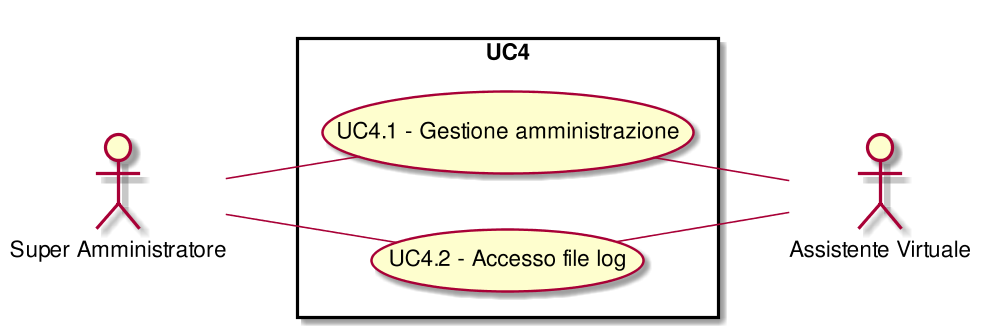
\includegraphics[width=\textwidth,height=\textheight,keepaspectratio]{images/UseCaseUC4.png}
\caption{UC4: Accesso funzionalità super amministratore}
\end{figure}
\begin{longtable}{l|p{10cm}}
\rowcolor[gray]{0.8} \multicolumn{2}{c}{} \\
\rowcolor[gray]{0.8} \multicolumn{2}{c}{\textbf{UC4 - Accesso funzionalità super amministratore}} \\
\rowcolor[gray]{0.8} \multicolumn{2}{c}{} \\
\hline
&\\
\textbf{Attori} & Super Amministratore.\\[7pt]
\textbf{Descrizione} & Il super amministratore può gestire gli amministratori ed accedere ai file \gl{log}.\\[7pt]
\textbf{Precondizione} & Il super amministratore si trova nella sezione adibita alla gestione.\\[7pt]
\textbf{Postcondizione} & Il super amministratore ha usufruito delle funzionalità di gestione.\\[7pt]
\textbf{Scenario principale} &\begin{enumerate}
\item  Il super amministratore può gestire gli amministratori del sistema;
\item  Il super amministratore può accedere ai file log.
\end{enumerate}
\\[7pt]\hline
\end{longtable}

\newpage\subsubsection{UC4.1: Gestione amministrazione}
\label{UC4.1}
\begin{figure}[h]
\centering
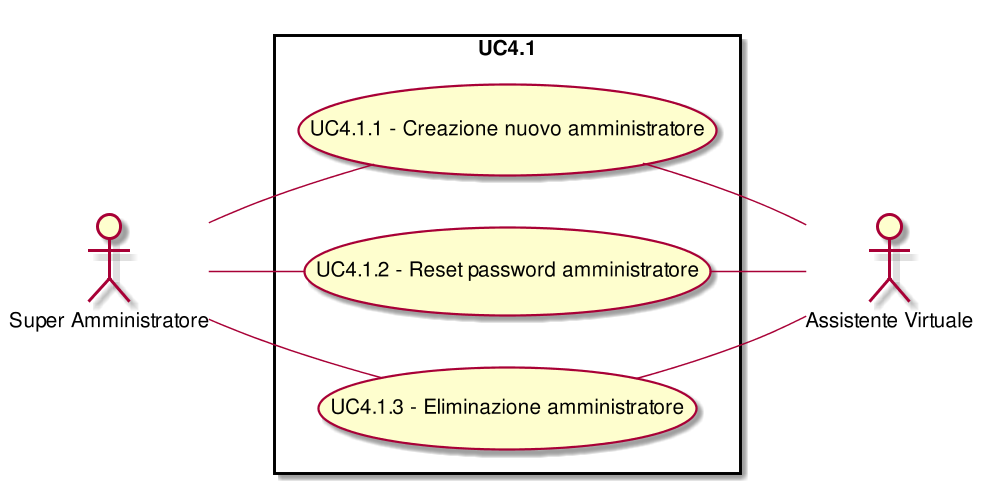
\includegraphics[width=\textwidth,height=\textheight,keepaspectratio]{images/UseCaseUC41.png}
\caption{UC4.1: Gestione amministrazione}
\end{figure}
\begin{longtable}{l|p{10cm}}
\rowcolor[gray]{0.8} \multicolumn{2}{c}{} \\
\rowcolor[gray]{0.8} \multicolumn{2}{c}{\textbf{UC4.1 - Gestione amministrazione}} \\
\rowcolor[gray]{0.8} \multicolumn{2}{c}{} \\
\hline
&\\
\textbf{Attori} & Assistente Virtuale, Super Amministratore.\\[7pt]
\textbf{Descrizione} & Il super amministratore può gestire gli amministratori del sistema.\\[7pt]
\textbf{Precondizione} & Il super amministratore si trova nella sezione per gestire gli amministratori.\\[7pt]
\textbf{Postcondizione} & Il super amministratore ha usufruito delle funzionalità per gestire gli amministratori.\\[7pt]
\textbf{Scenario principale} &\begin{enumerate}
\item  Il super amministratore può creare un nuovo amministratore;
\item  Il super amministratore può resettare la password degli amministratori;
\item  Il super amministratore può revocare i privilegi degli amministratori.
\end{enumerate}
\\[7pt]\hline
\end{longtable}

\newpage\subsubsection{UC4.1.1: Creazione nuovo amministratore}
\label{UC4.1.1}
\begin{figure}[h]
\centering
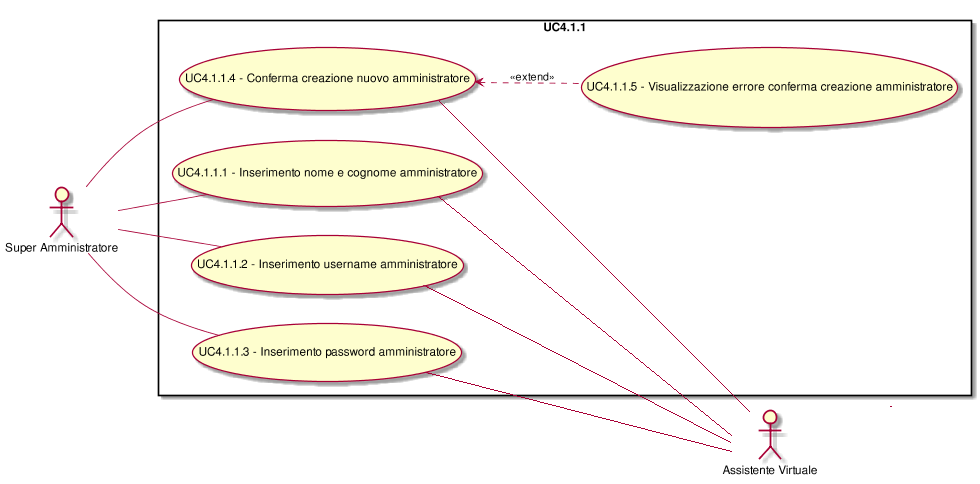
\includegraphics[width=\textwidth,height=\textheight,keepaspectratio]{images/UseCaseUC411.png}
\caption{UC4.1.1: Creazione nuovo amministratore}
\end{figure}
\begin{longtable}{l|p{10cm}}
\rowcolor[gray]{0.8} \multicolumn{2}{c}{} \\
\rowcolor[gray]{0.8} \multicolumn{2}{c}{\textbf{UC4.1.1 - Creazione nuovo amministratore}} \\
\rowcolor[gray]{0.8} \multicolumn{2}{c}{} \\
\hline
&\\
\textbf{Attori} & Assistente Virtuale, Super Amministratore.\\[7pt]
\textbf{Descrizione} & Il super amministratore può creare un nuovo amministratore.\\[7pt]
\textbf{Precondizione} & Il super amministratore si trova nella sezione per creare un nuovo amministratore.\\[7pt]
\textbf{Postcondizione} & Il super amministratore ha creato un nuovo amministratore.\\[7pt]
\textbf{Scenario principale} &\begin{enumerate}
\item  Il super amministratore può inserire nome e cognome dell'amministratore;
\item  Il super amministratore può inserire la password dell'amministratore;
\item  Il super amministratore può confermare il nuovo amministratore.
\end{enumerate}
\\[7pt]
\textbf{Scenari alternativi} & Il super amministratore visualizza un messaggio d'errore relativo alla conferma della creazione dell'amministratore.\\[7pt]\hline
\end{longtable}

\subsubsection{UC4.1.1.1: Inserimento nome e cognome amministratore}
\label{UC4.1.1.1}
\begin{longtable}{l|p{10cm}}
\rowcolor[gray]{0.8} \multicolumn{2}{c}{} \\
\rowcolor[gray]{0.8} \multicolumn{2}{c}{\textbf{UC4.1.1.1 - Inserimento nome e cognome amministratore}} \\
\rowcolor[gray]{0.8} \multicolumn{2}{c}{} \\
\hline
&\\
\textbf{Attori} & Assistente Virtuale, Super Amministratore.\\[7pt]
\textbf{Descrizione} & Il super amministratore può inserire nome e cognome del nuovo amministratore.\\[7pt]
\textbf{Precondizione} & Il super amministratore si trova nella sezione per creare un nuovo amministratore. \\[7pt]
\textbf{Postcondizione} & Il super amministratore ha inserito nome e cognome del nuovo amministratore.\\[7pt]
\textbf{Scenario principale} &Il super amministratore inserisce nome e cognome di un nuovo amministratore.\\[7pt]\hline
\end{longtable}

\subsubsection{UC4.1.1.2: Inserimento username amministratore}
\label{UC4.1.1.2}
\begin{longtable}{l|p{10cm}}
\rowcolor[gray]{0.8} \multicolumn{2}{c}{} \\
\rowcolor[gray]{0.8} \multicolumn{2}{c}{\textbf{UC4.1.1.2 - Inserimento username amministratore}} \\
\rowcolor[gray]{0.8} \multicolumn{2}{c}{} \\
\hline
&\\
\textbf{Attori} & Assistente Virtuale, Super Amministratore.\\[7pt]
\textbf{Descrizione} & Il super amministratore può inserire lo username di un nuovo amministratore.\\[7pt]
\textbf{Precondizione} & Il super amministratore si trova nella sezione per la creazione di un nuovo amministratore.\\[7pt]
\textbf{Postcondizione} & Il sistema ha ricevuto lo username di un nuovo amministratore.\\[7pt]
\textbf{Scenario principale} &Il super amministratore fornisce al sistema lo username di un nuovo amministratore.\\[7pt]\hline
\end{longtable}

\subsubsection{UC4.1.1.3: Inserimento password amministratore}
\label{UC4.1.1.3}
\begin{longtable}{l|p{10cm}}
\rowcolor[gray]{0.8} \multicolumn{2}{c}{} \\
\rowcolor[gray]{0.8} \multicolumn{2}{c}{\textbf{UC4.1.1.3 - Inserimento password amministratore}} \\
\rowcolor[gray]{0.8} \multicolumn{2}{c}{} \\
\hline
&\\
\textbf{Attori} & Assistente Virtuale, Super Amministratore.\\[7pt]
\textbf{Descrizione} & Il super amministratore può inserire la password di un nuovo amministratore.\\[7pt]
\textbf{Precondizione} & Il super amministratore si trova nella sezione per creare un nuovo amministratore. \\[7pt]
\textbf{Postcondizione} & Il super amministratore ha inserito la password del nuovo amministratore.\\[7pt]
\textbf{Scenario principale} &Il super amministratore inserisce la password per il nuovo amministratore.\\[7pt]\hline
\end{longtable}

\newpage\subsubsection{UC4.1.1.4: Conferma creazione nuovo amministratore}
\label{UC4.1.1.4}
\begin{longtable}{l|p{10cm}}
\rowcolor[gray]{0.8} \multicolumn{2}{c}{} \\
\rowcolor[gray]{0.8} \multicolumn{2}{c}{\textbf{UC4.1.1.4 - Conferma creazione nuovo amministratore}} \\
\rowcolor[gray]{0.8} \multicolumn{2}{c}{} \\
\hline
&\\
\textbf{Attori} & Assistente Virtuale, Super Amministratore.\\[7pt]
\textbf{Descrizione} & Il super amministratore può confermare i dati inseriti per la creazione di un nuovo amministratore.\\[7pt]
\textbf{Precondizione} & Il super amministratore si trova nella sezione per creare un nuovo amministratore. \\[7pt]
\textbf{Postcondizione} & Il super amministratore ha confermato la creazione del nuovo amministratore.\\[7pt]
\textbf{Scenario principale} &Il super amministratore conferma la creazione di un nuovo amministratore.\\[7pt]
\textbf{Scenari alternativi} & Il super amministratore non conferma di voler creare il nuovo amministratore. Il super amministratore viene rimandato alla pagina dedicata alla gestione degli amministratori.\\[7pt]\hline
\end{longtable}

\subsubsection{UC4.1.1.5: Visualizzazione errore conferma creazione amministratore}
\label{UC4.1.1.5}
\begin{longtable}{l|p{10cm}}
\rowcolor[gray]{0.8} \multicolumn{2}{c}{} \\
\rowcolor[gray]{0.8} \multicolumn{2}{c}{\textbf{UC4.1.1.5 - Visualizzazione errore conferma creazione amministratore}} \\
\rowcolor[gray]{0.8} \multicolumn{2}{c}{} \\
\hline
&\\
\textbf{Attori} & Assistente Virtuale, Super Amministratore.\\[7pt]
\textbf{Descrizione} & Il super amministratore può visualizzare un messaggio d'errore se ha comunicato dei dati non validi per la creazione di un nuovo amministratore.
I dati non validi sono: username già esistente.\\[7pt]
\textbf{Precondizione} & Il sistema ha ricevuto dati non validi.\\[7pt]
\textbf{Postcondizione} & Il sistema mostra un messaggio d'errore.\\[7pt]
\textbf{Scenario principale} &Il super amministratore visualizza un messaggio d'errore.\\[7pt]\hline
\end{longtable}

\newpage\subsubsection{UC4.1.2: Reset password amministratore}
\label{UC4.1.2}
\begin{figure}[h]
\centering
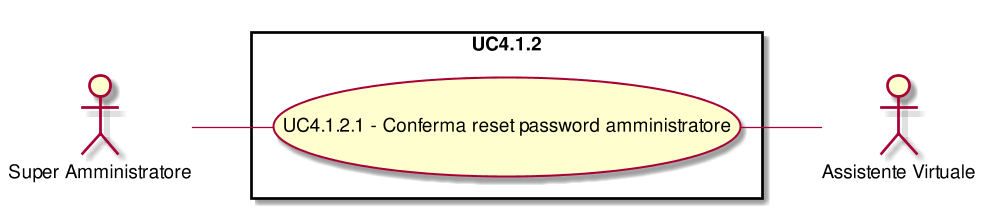
\includegraphics[width=\textwidth,height=\textheight,keepaspectratio]{images/UseCaseUC412.png}
\caption{UC4.1.2: Reset password amministratore}
\end{figure}
\begin{longtable}{l|p{10cm}}
\rowcolor[gray]{0.8} \multicolumn{2}{c}{} \\
\rowcolor[gray]{0.8} \multicolumn{2}{c}{\textbf{UC4.1.2 - Reset password amministratore}} \\
\rowcolor[gray]{0.8} \multicolumn{2}{c}{} \\
\hline
&\\
\textbf{Attori} & Assistente Virtuale, Super Amministratore.\\[7pt]
\textbf{Descrizione} & Il super amministratore può resettare la password dell'amministratore.\\[7pt]
\textbf{Precondizione} & Il super amministratore si trova nella sezione per resettare la password di un amministratore.\\[7pt]
\textbf{Postcondizione} & Il super amministratore ha resettato la password dell'amministratore.\\[7pt]
\textbf{Scenario principale} &\begin{enumerate}
\item  Il super amministratore può inserire la nuova password dell'amministratore;
\item  il super amministratore può confermare la nuova password dell'amministratore;
\item  il super amministratore può confermare il reset della password.
\end{enumerate}
\\[7pt]
\textbf{Scenari alternativi} & Il super amministratore visualizza un messaggio d'errore relativo al reset della password dell'amministratore.\\[7pt]\hline
\end{longtable}

\subsubsection{UC4.1.2.1: Conferma reset password amministratore}
\label{UC4.1.2.1}
\begin{longtable}{l|p{10cm}}
\rowcolor[gray]{0.8} \multicolumn{2}{c}{} \\
\rowcolor[gray]{0.8} \multicolumn{2}{c}{\textbf{UC4.1.2.1 - Conferma reset password amministratore}} \\
\rowcolor[gray]{0.8} \multicolumn{2}{c}{} \\
\hline
&\\
\textbf{Attori} & Assistente Virtuale, Super Amministratore.\\[7pt]
\textbf{Descrizione} & Il super amministratore può confermare il reset della password.\\[7pt]
\textbf{Precondizione} & Il super amministratore si trova nella sezione per confermare il reset della password dell'amministratore.\\[7pt]
\textbf{Postcondizione} & Il super amministratore ha confermato il reset della password dell'amministratore.\\[7pt]
\textbf{Scenario principale} &Il super amministratore conferma il reset della password dell'amministratore.\\[7pt]
\textbf{Scenari alternativi} & Il super amministratore non conferma di voler resettare la password dell'amministratore. Il super amministratore viene rimandato alla pagina dedicata alla gestione degli amministratori.\\[7pt]\hline
\end{longtable}

\subsubsection{UC4.1.3: Eliminazione amministratore}
\label{UC4.1.3}
\begin{figure}[h]
\centering
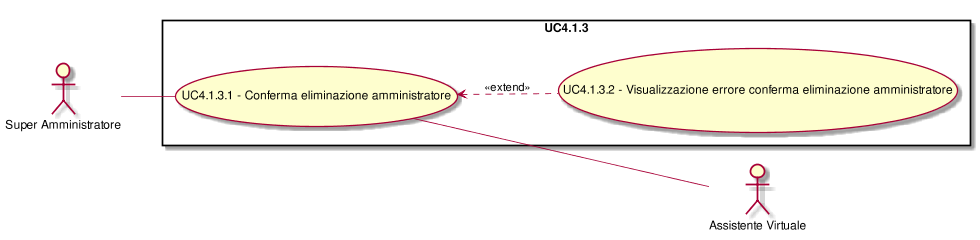
\includegraphics[width=\textwidth,height=\textheight,keepaspectratio]{images/UseCaseUC413.png}
\caption{UC4.1.3: Eliminazione amministratore}
\end{figure}
\begin{longtable}{l|p{10cm}}
\rowcolor[gray]{0.8} \multicolumn{2}{c}{} \\
\rowcolor[gray]{0.8} \multicolumn{2}{c}{\textbf{UC4.1.3 - Eliminazione amministratore}} \\
\rowcolor[gray]{0.8} \multicolumn{2}{c}{} \\
\hline
&\\
\textbf{Attori} & Assistente Virtuale, Super Amministratore.\\[7pt]
\textbf{Descrizione} & Il super amministratore può rimuovere un amministratore dal sistema\\[7pt]
\textbf{Precondizione} & Il super amministratore si trova nella sezione per l'eliminazione di un amministratore.\\[7pt]
\textbf{Postcondizione} & Il super amministratore ha eliminato un amministratore dal sistema.\\[7pt]
\textbf{Scenario principale} &\begin{enumerate}
\item  Il super amministratore può eliminare un amministratore;
\item  il super amministratore può confermare l'eliminazione dell'amministratore.
\end{enumerate}
\\[7pt]
\textbf{Scenari alternativi} & Il super amministratore visualizza un messaggio d'errore relativo alla revoca dei privilegi dell'amministratore.\\[7pt]\hline
\end{longtable}

\subsubsection{UC4.1.3.1: Conferma eliminazione amministratore}
\label{UC4.1.3.1}
\begin{longtable}{l|p{10cm}}
\rowcolor[gray]{0.8} \multicolumn{2}{c}{} \\
\rowcolor[gray]{0.8} \multicolumn{2}{c}{\textbf{UC4.1.3.1 - Conferma eliminazione amministratore}} \\
\rowcolor[gray]{0.8} \multicolumn{2}{c}{} \\
\hline
&\\
\textbf{Attori} & Assistente Virtuale, Super Amministratore.\\[7pt]
\textbf{Descrizione} & Il super amministratore può confermare l'eliminazione di un amministratore.\\[7pt]
\textbf{Precondizione} & Il super amministratore ha comunicato l'amministratore che vuole eliminare.\\[7pt]
\textbf{Postcondizione} & Il super amministratore ha eliminato un amministratore.\\[7pt]
\textbf{Scenario principale} &Il super amministratore conferma di volere eliminare un amministratore.\\[7pt]
\textbf{Scenari alternativi} & Il super amministratore non conferma di voler eliminare l'amministratore. Il super amministratore viene rimandato alla pagina dedicata alla gestione degli amministratori.\\[7pt]\hline
\end{longtable}

\subsubsection{UC4.1.3.2: Visualizzazione errore conferma eliminazione amministratore}
\label{UC4.1.3.2}
\begin{longtable}{l|p{10cm}}
\rowcolor[gray]{0.8} \multicolumn{2}{c}{} \\
\rowcolor[gray]{0.8} \multicolumn{2}{c}{\textbf{UC4.1.3.2 - Visualizzazione errore conferma eliminazione amministratore}} \\
\rowcolor[gray]{0.8} \multicolumn{2}{c}{} \\
\hline
&\\
\textbf{Attori} & Assistente Virtuale, Super Amministratore.\\[7pt]
\textbf{Descrizione} & L'amministratore può visualizzare un messaggio d'errore se ha comunicato dei dati non validi per l'eliminazione di un amministratore.
I dati non validi sono: username amministratore inesistente.\\[7pt]
\textbf{Precondizione} & Il sistema ha ricevuto dati non validi.\\[7pt]
\textbf{Postcondizione} & Il sistema mostra un messaggio d'errore.\\[7pt]
\textbf{Scenario principale} &Il super amministratore visualizza un messaggio d'errore.\\[7pt]\hline
\end{longtable}

\subsubsection{UC4.2: Accesso file log}
\label{UC4.2}
\begin{longtable}{l|p{10cm}}
\rowcolor[gray]{0.8} \multicolumn{2}{c}{} \\
\rowcolor[gray]{0.8} \multicolumn{2}{c}{\textbf{UC4.2 - Accesso file log}} \\
\rowcolor[gray]{0.8} \multicolumn{2}{c}{} \\
\hline
&\\
\textbf{Attori} & Assistente Virtuale, Super Amministratore.\\[7pt]
\textbf{Descrizione} & Il super amministratore può accedere ai file log.\\[7pt]
\textbf{Precondizione} & Il super amministratore si trova nella sezione adibita alla visualizzazione dei file log.\\[7pt]
\textbf{Postcondizione} & Il super amministratore ha fatto accesso ai file log\\[7pt]
\textbf{Scenario principale} &Il super amministratore accede e visualizza i file log.\\[7pt]\hline
\end{longtable}
\newpage
\subsection{UC5: Comunicazione non comprensibile}
\label{UC5}
\begin{longtable}{l|p{10cm}}
\rowcolor[gray]{0.8} \multicolumn{2}{c}{} \\
\rowcolor[gray]{0.8} \multicolumn{2}{c}{\textbf{UC5 - Comunicazione non comprensibile}} \\
\rowcolor[gray]{0.8} \multicolumn{2}{c}{} \\
\hline
&\\
\textbf{Attori} & Assistente Virtuale.\\[7pt]
\textbf{Descrizione} & Il sistema richiederà all'utente una chiarimento nel caso in cui non riesca a interpretare la sua risposta.\\[7pt]
\textbf{Precondizione} & Il sistema non è riuscito ad interpretare una comunicazione dell'utente.\\[7pt]
\textbf{Postcondizione} & Il sistema comunica l'errore richiedendo nuovamente l'informazione all'utente.\\[7pt]
\textbf{Scenario principale} &L'utente comunica nuovamente l'informazione non compresa dal sistema.\\[7pt]\hline
\end{longtable}

\subsection{UC6: Scadenza timeout input}
\label{UC6}
\begin{longtable}{l|p{10cm}}
\rowcolor[gray]{0.8} \multicolumn{2}{c}{} \\
\rowcolor[gray]{0.8} \multicolumn{2}{c}{\textbf{UC6 - Scadenza timeout input}} \\
\rowcolor[gray]{0.8} \multicolumn{2}{c}{} \\
\hline
&\\
\textbf{Attori} & Assistente Virtuale.\\[7pt]
\textbf{Descrizione} & L'utente, per ogni interazione con il sistema, ha un tempo limitato di risposta. Scaduto questo lasso di tempo l'utente visualizzerà un opportuno messaggio, attraverso il quale potrà tornare alla schermata precedente.\\[7pt]
\textbf{Precondizione} & L'utente non ha interagito con il sistema entro il tempo prestabilito di risposta.\\[7pt]
\textbf{Postcondizione} & L'utente ha visualizzato il messaggio oppure il sistema si è disattivato.\\[7pt]
\textbf{Scenario principale} &L'utente visualizza un messaggio opportuno. \\[7pt]
\textbf{Scenari alternativi} & Nel caso in cui l'utente non confermi la sua presenza il sistema si disattiva.\\[7pt]\hline
\end{longtable}
